\documentclass{article}
\usepackage{cite}
\usepackage{amsmath,amssymb,amsfonts}
\usepackage{algorithmic}
\usepackage{graphicx}
\usepackage{textcomp}
\usepackage{hyperref}
\usepackage{footnotebackref}
\usepackage{array}
\usepackage[ruled,vlined]{algorithm2e}
\usepackage{enumitem}
\usepackage{booktabs}
\usepackage{multicol}
\usepackage{url}
\usepackage[acronym]{glossaries}
\usepackage{caption}
\captionsetup[table]{font=small, skip=5pt}
\hypersetup{
    colorlinks=true,
    linkcolor=blue,
    filecolor=magenta,      
    urlcolor=blue,
}
\usepackage{xcolor}
\def\BibTeX{{\rm B\kern-.05em{\sc i\kern-.025em b}\kern-.08em
    T\kern-.1667em\lower.7ex\hbox{E}\kern-.125emX}}

\makeglossaries

\newacronym{ffnn}{FFNN}{Feed Forward Neural Networks}
\newacronym{cnn}{CNN}{Convolutional Neural Network}
\newacronym{mmnn}{MMNN}{Multi Modal Neural Network}
\newacronym{m}{m}{Min Value}
\newacronym{M}{M}{Max Value}
\newacronym{s}{s}{Step}

\newacronym{IN}{IN}{Input Layer}
\newacronym{OUT}{OUT}{Output Layer}
\newacronym{DN}{DN}{Dense Layer}
\newacronym{C1D}{C1D}{1D Convolution Layer}
\newacronym{BN}{BN}{Batch Normalization Layer}
\newacronym{DR}{DR}{Dropout Layer}
\newacronym{RL}{RL}{Relu Activation}
\newacronym{MP1D}{MP1D}{MaxPool1D Layer}
\newacronym{GAP1D}{GAP1D}{GlobalAveragePooling1D Layer}

\newacronym{bs}{bs}{Base Pair}
\newacronym{ENCODE}{ENCODE}{Encyclopedia of DNA Elements}
\newacronym{UCSC}{UCSC}{University of California, Santa Cruz}
\newacronym{FANTOM}{FANTOM}{Functional Annotation Of the Mammalian genome}
\newacronym{HPC}{HPC}{High Performance Computing}
\newacronym{TPM}{TPM}{Tags Per Million}
\newacronym{MIC}{MIC}{Maximum Coefficient Of Information}
\newacronym{ST}{ST}{Statistically Indistinguishable}

\newacronym{AE-IE}{AE-IE}{active enhancers vs inactive enhancers}
\newacronym{AP-IP}{AP-IP}{active promoters vs inactive promoters}

\begin{document}

\title{Prediction of regulatory regions in a specific cell line using Deep Learning Techniques}
\author{{1\textsuperscript{st} Giuseppe Bonura}\\
\textit{University of Milan}\\
\textit{Department of Computer Science}\\
\url{giuseppe.bonura@studenti.unimi.it}}

\maketitle

\section{Introduction}
\label{sec:introduction}
In a very short interval, “bioinformatics” has become an extremely active research field. Although it began with sequence comparison (which is a sub branch of the study of the non randomness of DNA sequences), it now encompasses a far wider spread of activity, which truly epitomizes modern scientific research. It's highly interdisciplinary field mainly involving molecular biology and genetics, computer science, mathematics and statistics. It uses computer programs for a variety of applications, including determining gene and protein functions, establishing evolutionary relationships, and predicting the three-dimensional shapes of proteins.
\newline
\noindent
In this project, the focus is mainly on the DNA sequence and the human genome, in fact it's purpose is to analyze regulatory regions in \textbf{H1} cell line and determine which regions are active and which are not.

\subsection{What are regulatory regions?}
Less than 2/3\% of the DNA is believed to encode useful information. The remain percentage sometimes called “junk” DNA, has no apparent function. Of the 2/3\% of functional DNA, the majority specifies genes—regions of the DNA comprising two parts, a regulatory region or promoter and a coding region.
The regulatory region is partly responsible for specifying the conditions under which the gene product is produced, or the degree to which it's produced. The coding region specifies the functional molecular product or products often a protein, but sometimes an RNA (ribonucleic acid). For protein-coding genes, the coding region specifies the amino-acid sequence of the protein. However, the protein is not constructed directly from the DNA. Instead, the DNA is transcribed into an RNA intermediate, called messenger RNA (mRNA), which is then translated into a protein. 
\newline
\newline
\noindent
In Section \ref{sec:Models} we will provide an overview of the models evaluated on the aforementioned tasks, along with the corresponding explored hyper-parameter spaces. In Section \ref{sec:Experimental_Setup} we will discuss details pertaining to the execution of the experiments and to the data. Finally, in Section \ref{sec:Results} we will present the results of the experiments and their implications.

\section{Models}
\label{sec:Models}
In this work, deep neural networks are build for binary classification useful for predicting the activity of regulatory regions in the H1 cell line. They have been made three different types of deep neural network architectures, and the adjustment of parameters in each neural networks is a very complex and expensive task, for this reason, in order to have a sufficiently truthful model with consistent parameters, it was used KerasTuner, which is an easy-to-use, scalable hyperparameter optimization framework that solves the pain points of hyperparameter search.
\begin{itemize}
  \item Multilayer perceptron or Feed Forward Neural Network
  \item Convolutional Neural Network 
  \item Multimodal Neural Network
\end{itemize}
The supervised approach was used for all models. That supervised learning algorithms are, roughly speaking, learning algorithms that learn to associate some input with some output, given training set of examples of inputs $x$ and outputs $y$. In many cases the outputs $y$ may be difficult to collect automatically and must be provided by a human "supervisor". Let's see in detail of each model.

\subsection{Artificial Neural Network}
Artificial neural networks are popular machine learning techniques that simulate the mechanism of learning in biological organisms. The human nervous system contains cells, which are referred to as neurons.\cite{Aggarwal2018} Generally artificial neural networks are very simple and consist of only one layer between the network input and output. Similarly, it's architectural simplicity doesn't allow us to approximate very complex mathematical functions. In this regard, what are known as deep neural networks have been introduced, i.e. neural networks that have a greater number of 2 hidden layers between the input and output layers. These models are called \textbf{feed-forward} because information flows through the function being evaluated from $x$, through the intermediate computations used to define $f$, and finally to the output $y$. There are no cycles or loops in the network.\cite{goodfellow2016deep} All neural networks used in this work are classified as a feed-forward neural network.

\subsection{Multilayer perceptron}
Multilayer neural networks contain multiple computational layers; the additional intermediate layers (between input and output) are referred to as hidden layers because the computations performed are not visible to the user.
The specific architecture of multilayer neural networks is referred to as feed-forward networks, because successive layers feed into one another in the forward direction from input to output. The default architecture of feed-forward networks assumes that all nodes in one layer are connected to those of the next layer. Therefore, the architecture of the neural network is almost fully defined, once the number of layers, the number/type of nodes in each layer and type of activation function have been defined.\cite{Aggarwal2018}

\begin{table}[!ht]
\begin{center}
\begin{tabular}{ |c|c|c|c| }
 \hline
 \multicolumn{4}{|c|}{FFNN Summary} \\
 \hline
    N.Layers & Layers Type & N.Neurons & Activation\\
 \hline 
    Input & \href{https://www.tensorflow.org/api_docs/python/tf/keras/layers/InputLayer}{Input} & 58 & - \\
    1,2 & \href{https://www.tensorflow.org/api_docs/python/tf/keras/layers/InputLayer}{Dense} & 160 &   \href{https://www.tensorflow.org/api_docs/python/tf/keras/layers/ReLU}{ReLu}\\
    3,4,5,6 &   \href{https://www.tensorflow.org/api_docs/python/tf/keras/layers/InputLayer}{Dense} & 208 &   \href{https://www.tensorflow.org/api_docs/python/tf/keras/layers/ReLU}{ReLu}\\
    Output  &   \href{https://www.tensorflow.org/api_docs/python/tf/keras/layers/InputLayer}{Dense} & 1 &   \href{https://www.tensorflow.org/api_docs/python/tf/keras/activations/sigmoid}{Sigmoid}\\
 \hline
\end{tabular}
\caption{\label{tab:FFNN_Summary} \acrshort{ffnn}  Architecture.}
\end{center}
\end{table}

\begin{figure}[!ht]
    \centering
    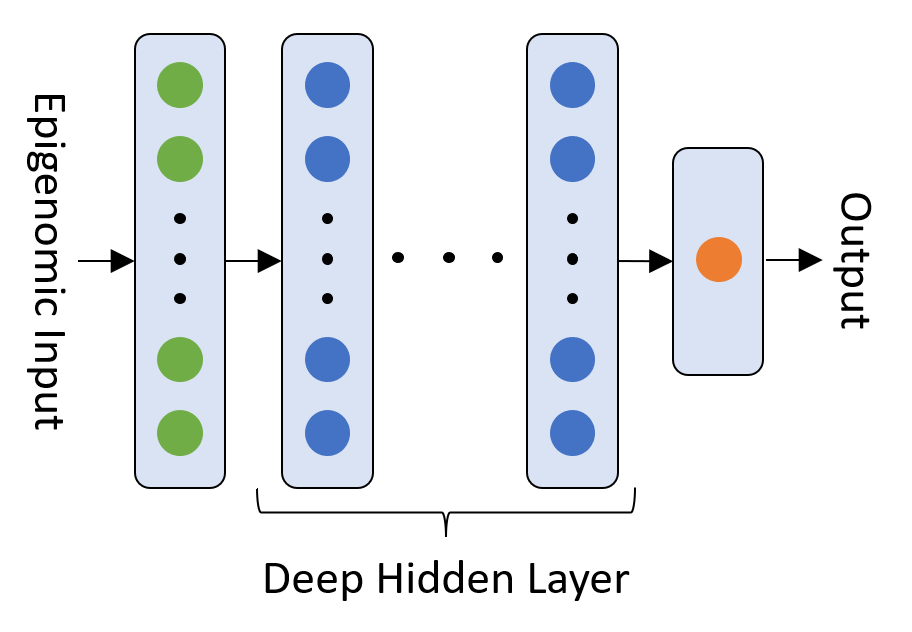
\includegraphics[width=6cm]{image/FFNN_Diagram.PNG}
    \caption{\acrshort{ffnn} Network Diagram}
    \label{fig:FFNN_Diagram}
\end{figure}

\centerline{The hyperparameter space used for the tuner the \acrshort{ffnn} are:}

\begin{table}[!ht]
\begin{center}
\begin{tabular}{||c | c | c ||} 
 \hline
 Parameter Name & Hyperparameter Values & Result\\ [0.5ex] 
 \hline\hline
 num\_layers & \acrshort{m}=2 \acrshort{M}=6 \acrshort{s}=1 & 6 \\ 
 \hline
 n\_neurons0 & \acrshort{m}=32 \acrshort{M}=256 \acrshort{s}=32 & 160 \\
 \hline
 n\_neurons1 & \acrshort{m}=16 \acrshort{M}=256 \acrshort{s}=16 & 208\\
 \hline
 learning\_rate & \{1e-2, 1e-4\} & 1e-2\\
 \hline
\end{tabular}
\caption{\label{tab:FFNN_Hyperparameter} \acrshort{ffnn} Hyperparameter Space.}
\end{center}
\end{table}

\newpage
\subsection{Convolutional Neural Network }
Convolutional neural networks, or CNNs, are a specialized kind of neural network for processing data that has a known grid-like topology. Examples include time-series data, which can be thought of as a 1-D grid taking samples at regular time intervals, and image data,which can be thought of as a 2-D grid of pixels. Convolutional networks have been tremendously successful in practical applications. The name “convolutional neural network” indicates that the network employs a mathematical operation called convolution. Convolution is a specialized kind of linear operation. Convolutional networks are simply neural networks that use convolution in place of general matrix multiplication in at least one of their layers.\cite{goodfellow2016deep} We will note that within the model of this \acrshort{cnn} there will not only be the convolution layer, but there will be more layers that we will briefly describe:

\begin{itemize}
    \item \textbf{Input layer:\footnote{\url{https://www.tensorflow.org/api_docs/python/tf/keras/layers/InputLayer}}} This layer represent the entry point of a neural network. Its shape should be equal to the shape of the inputs. In our case the shape is determined by the window size of nucleotides considered.
    \item \textbf{Conv1D:\footnote{\url{https://www.tensorflow.org/api_docs/python/tf/keras/layers/Conv1D}}} This layer creates a convolution kernel that is convolved with the layer input over a single spatial (or temporal) dimension to produce a tensor of outputs.
    \item \textbf{Batch Normalization:\footnote{\url{https://www.tensorflow.org/api_docs/python/tf/keras/layers/BatchNormalization}}} This layer applies a transformation that maintains the mean output close to 0 and the output standard deviation close to 1. The activation function is applied after each layer of batch normalization.
    \item \textbf{Activation Function:\footnote{\url{https://www.tensorflow.org/api_docs/python/tf/keras/layers/Activation}}} An activation function in a neural network defines how the weighted sum of the input is transformed into an output from a node or nodes in a layer of the network. The ReLu function, acronym for rectifier linear unit, was used for this model. It's a very simple function to calculate: it flattens the answer to all negative values to zero, while leaving everything unchanged for values that are equal or greater than zero.
    \item \textbf{Dropout:\footnote{\url{https://www.tensorflow.org/api_docs/python/tf/keras/layers/Dropout}}} The dropout is a technique that allows the deactivation of a percentage of neurons within each hidden layer, thus modifying the topology (in terms of neurons). For each epoch of training, one chooses (randomly) which neurons to keep and which ones to discard and the resulting network is trained. The procedure is then repeated, keeping and discarding different neurons at each epoch: once the network is deemed ready, the original network is taken and the weights coming out of the previously deactivated neurons are adjusted.
    \item \textbf{MaxPooling1D:\footnote{\url{https://www.tensorflow.org/api_docs/python/tf/keras/layers/MaxPool1D}}} This layer allows us to reduce the dimensionality of the input by concentrating everything in a single sample and aggregating the weight values using a specific function, in this case the maximum value.
    \item \textbf{GlobalMaxPooling1D:\footnote{\url{https://www.tensorflow.org/api_docs/python/tf/keras/layers/GlobalMaxPool1D}}} This layer is similar to MaxPooling1D, but it aggregates an entire feature map in one value.
    \item \textbf{Dense:\footnote{\url{https://www.tensorflow.org/api_docs/python/tf/keras/layers/Dense}}} Dense layer is a standard fully connected layer.
\end{itemize}

\noindent
In this project it has been used providing in input layer a sequences of data in matrix form. Let's see in detail the architecture of the \acrshort{cnn} designed. 

\begin{table}[!ht]
\begin{center}
\begin{tabular}{ |c|c|c|c|c| }
 \hline
 \multicolumn{5}{|c|}{CNN Summary} \\
 \hline
    N.Layers & Layers Type & Filters Shape & Kernel Size & Activation\\
 \hline
    Input   &   \acrshort{IN}   &   [(256, 4)]  &   -   &   -   \\
    1   &   \acrshort{C1D}, \acrshort{BN}, \acrshort{RL}, \acrshort{DR} &  [(256, 4)] & 8 &   ReLu\\
    2   &   \acrshort{C1D}, \acrshort{BN}, \acrshort{RL}, \acrshort{DR}, \acrshort{MP1D} &  [(242, 64)] & 8 &   ReLu\\
    3   &   \acrshort{C1D}, \acrshort{BN}, \acrshort{RL}, \acrshort{DR} & [(120, 32)] & 2 &   ReLu\\
    4   &   \acrshort{C1D}, \acrshort{BN}, \acrshort{RL}, \acrshort{DR}, \acrshort{MP1D} & [(119, 32)] & 2 &   ReLu\\
    5   &   \acrshort{C1D}, \acrshort{BN}, \acrshort{RL}, \acrshort{DR} & [(59, 32)] & 2 &   ReLu\\
    6   &   \acrshort{GAP1D}, \acrshort{BN}, \acrshort{DR} & 32 & - &   -\\
    7   &   \acrshort{DN} & 80 & - &   -\\
    Output  &   \acrshort{OUT}  & 1 & - &   Sigmoid\\
 \hline
\end{tabular}
\caption{\label{tab:CNN_Summary} \acrshort{cnn}  Architecture.}
\end{center}
\end{table}

\begin{figure}[!ht]
    \centering
    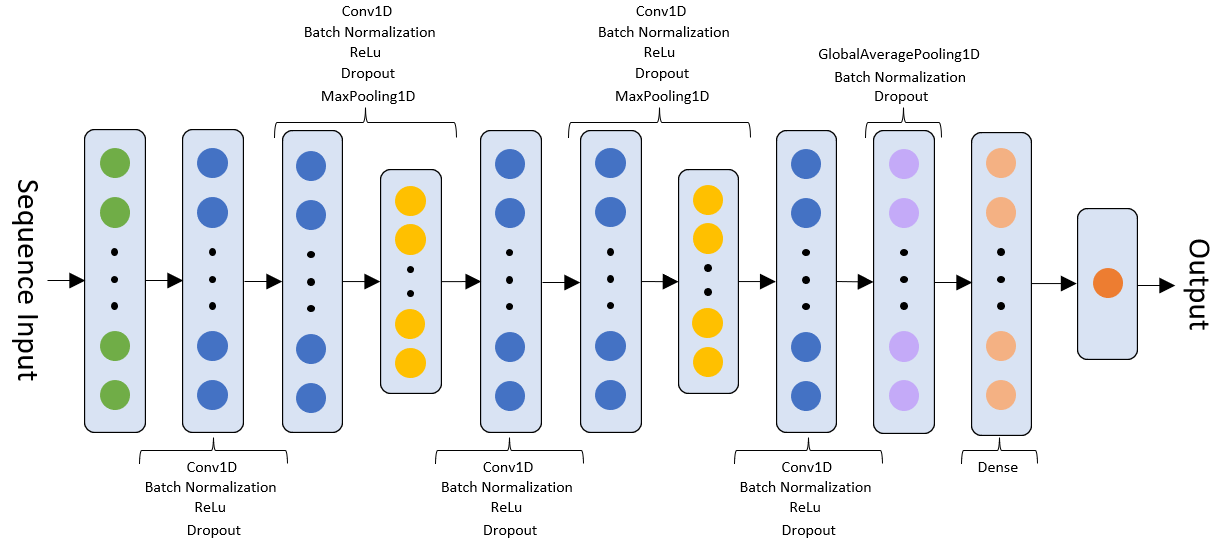
\includegraphics[width=12cm]{image/CNN_Diagram.PNG}
    \caption{\acrshort{cnn} Network Diagram}
    \label{fig:CNN_Diagram}
\end{figure}

\centerline{The hyperparameter space used for the tuner of the \acrshort{cnn} are:}

\begin{table}[!ht]
\begin{center}
\begin{tabular}{||c | c | c ||} 
 \hline
 Parameter Name & Hyperparameter Values & Result\\ [0.5ex] 
 \hline\hline
 num\_conv\_layers & \acrshort{m}=2 \acrshort{M}=8 \acrshort{s}=1 &  5\\ 
    \hline
    kernel\_size\_0 & \acrshort{m}=5 \acrshort{M}=8 \acrshort{s}=1 &  8\\ 
    \hline
    n\_filter\_0 & \acrshort{m}=32 \acrshort{M}=128 \acrshort{s}=32 & 64\\
    \hline
    drop\_rate\_input & \acrshort{m}=0 \acrshort{M}=0.5 \acrshort{s}=1 & 0.19335805735959433\\
    \hline
    drop\_rate\_out & \acrshort{m}=0 \acrshort{M}=0.5 \acrshort{s}=1 & 0.39499479777555135\\
    \hline
    kernel\_size\_1 & \acrshort{m}=2 \acrshort{M}=10 \acrshort{s}=1 & 2\\ 
    \hline
    n\_filter\_1 & \acrshort{m}=16 \acrshort{M}=128 \acrshort{s}=16 & 32\\
    \hline
    n\_filter\_output & \acrshort{m}=16 \acrshort{M}=128 \acrshort{s}=16 & 80\\
    \hline
    learning\_rate & \{1e-2, 1e-4\} & 1e-2\\
    \hline
\end{tabular}
\caption{\label{tab:CNN_Hyperparameter} \acrshort{cnn} Hyperparameter Space.}
\end{center}
\end{table}

\subsection{Multimodal Neural Network}
Multimodal neural networks are precisely networks that give us the possibility of combining two or more deep neural networks, in order to exploit the potential of the latter.
In the real world, information comes from heterogeneous sources represented in different ways. Obviously this difference in data representation provides different statistics and properties. The main objective of multimodal networks is therefore to exploit as much as possible the properties and benefits provided by each single neural network.
In the project it was therefore planned to bring together the result of the two networks in a junction layer followed by a dense layer. This approach will therefore help us in increasing the degree of prediction of the task by combining epigenomic data, managed by the \acrshort{ffnn} network, and genomic data (sequence data), managed by the \acrshort{cnn} network.
\begin{table}[!ht]
\begin{center}
\begin{tabular}{ |c|c|c|c|c| }
 \hline
 \multicolumn{5}{|c|}{MMNN Summary} \\
 \hline
    N.Layers & Network Type & Layers Type & N.Neurons & Activation\\
 \hline
    Input 1 &  FFNN & - & - &   -\\
    Input 2 &  CNN & - & - &   -\\
    1   & - & Concatenate & - &   -\\
    2   & - & Dense & 64 &   ReLu\\
    Output  & - & Dense & 1 &   Sigmoid\\
 \hline
\end{tabular}
\caption{\label{tab:MMNN_Summary} \acrshort{mmnn}  Architecture.}
\end{center}
\end{table}

\begin{figure}[!ht]
    \centering
    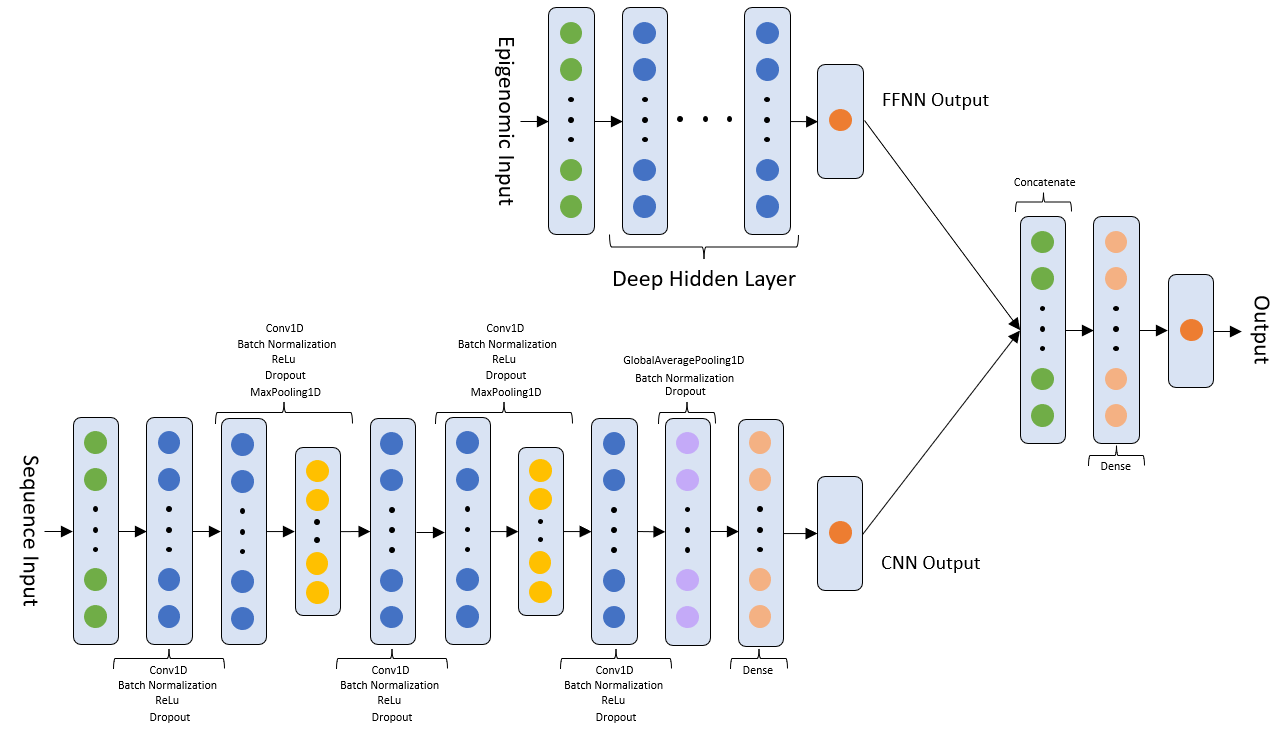
\includegraphics[width=11cm]{image/MMNN_Diagram.PNG}
    \caption{\acrshort{mmnn} Network Diagram}
    \label{fig:MMNN_Diagram}
\end{figure}

\noindent
The hyperparameter space used for the tuner of the \acrshort{mmnn} are show in Table \ref{tab:MMNN_Hyperparameter}. There are also some parameters common to all three networks visible in the Table \ref{tab:Common_Hyperparameter}.

\begin{table}[!ht]
\begin{center}
\begin{tabular}{||c | c | c ||} 
 \hline
 Parameter Name & Hyperparameter Values & Result\\ [0.5ex] 
 \hline\hline
 n\_neurons\_concat & \acrshort{m}=32 \acrshort{M}=256 \acrshort{s}=32 & 64\\
 \hline
 learning\_rate & \{1e-2, 1e-4\} & 1e-2\\
 \hline
\end{tabular}
\caption{\label{tab:MMNN_Hyperparameter} \acrshort{mmnn} Hyperparameter Space.}
\end{center}
\end{table}

\begin{table}[!ht]
\begin{center}
\begin{tabular}{||c | c ||} 
 \hline
 Hyperparameter & Values\\ [0.5ex] 
 \hline\hline
 Loss Function & Binary Crossentropy   \\
 \hline
 Optimizer & Nadam  \\
 \hline
 Epochs & 1000  \\
 \hline
 Early Stopping Patience & 2    \\
 \hline
 Early Stopping Min Delta & 0.001   \\
 \hline
\end{tabular}
\caption{\label{tab:Common_Hyperparameter} Common Hyperparameter Value.}
\end{center}
\end{table}

\section{Experimental setup}
\label{sec:Experimental_Setup}
The experiment was performed on two machine, and consist in the study of two tasks:
\begin{itemize}
    \item active enhancers vs inactive enhancers (AEvsIE)
    \item active promoters vs inactive promoters (APvsIP)
\end{itemize}
in the H1 \cite{hergeth2015h1} cell line, on the HG38\footnote{\url{https://genome-euro.ucsc.edu/cgi-bin/hgGateway?redirect=manual&source=genome.ucsc.edu}} dataset.

\newpage
\subsection{The considered tasks}
\label{sec:Task}
The first and main machine used for performed the task is Colab\footnote{Free hosted Jupyter notebook service by Google, that providing computing resources including GPUs. \url{https://research.google.com/colaboratory/faq.html}} and the second is a personal notebook with this HW and SW characteristics:
\begin{itemize}
    \item[-] Intel i5-8250U
    \item[-] 16 GB of Ram
    \item[-] Windows 10 Home x64
    \item[-] Editor Vs-Code\footnote{\url{https://code.visualstudio.com/}} 1.63.2 
    \item[-] Python Virtual Env With v3.7.4\footnote{\url{https://www.python.org/downloads/release/python-374/}}
\end{itemize}
The two tasks considered aim to study the activity of enhancer and promoter regions in the H1 cell line. Each task is executed using a single fix dimension of window sizes set to: 256\acrshort{bs} (given the limited resources in the development environment, a higher number of windows would have caused the instance to time out and not complete tasks). The chosen window size determines the relative number of nucleotides associated with the enhancer or promoter region considered. All the project phases have been divided into three macro areas. In a first phase, a binary exploration of the data was performed in order to determine the appropriate threshold values for the assigned cell line. In the second stage the hyperparameters were tuned (using Keras Tuner\footnote{\url{https://keras.io/keras_tuner/}}) for each network model in personal computer, then identified and cached the results. The third e last phase is the training of the model, that was performed on Colab with feature selection using boruta with the maximum number set to 30 iterations to avoid execution time too long and sending Colab into time-out without having completed the tasks in development.

\subsection{Dataset source}
\label{sec:Dataset}
The data used for the experiment are divided into:
\begin{enumerate}
    \item Epigenomic Data  
    \item Sequence Data
    \item Labels
\end{enumerate}
Epigenomic data was retrieved from \acrshort{ENCODE}\footnote{\url{https://www.encodeproject.org/}}, that is a consortium formed by research groups, whose collaboration aims to create a complete list of functional elements in the human genome, including elements that act at the protein and RNA levels, and regulatory elements that control cells and circumstances in which a gene is active.
\newline
The sequence data was recovered from the \acrshort{UCSC} Genome Browser\footnote{\url{https://genome-euro.ucsc.edu/index.html}}. This is a web site where members of the International Human Genome Project consortium give the possibility to publicly access and download the data of the human genome giving the possibility to have a graphic visualization tool.
\newline
As for the labels used for training and testing of neural networks, the data used was taken from FANTOM5. FANTOM5 is the evolution of the \acrshort{FANTOM}\footnote{\url{https://fantom.gsc.riken.jp/}} project, that is an international project, born around the 2000s aiming at identifying all functional elements in mammalian genomes.
\newline
Fortunately, the hard work to retrieve the epigenomic data from \acrshort{ENCODE}, retrieving the labels from \acrshort{FANTOM} and querying the terabytes of bigwig files has already been done using an \acrshort{HPC}. Some python packages have been made available which are useful for speeding up the execution of the project.
\begin{itemize}
    \item epigenomic\_data\footnote{\url{https://github.com/AnacletoLAB/epigenomic_dataset}}: Is a package developed by the PhD students of Anacleto Lab\footnote{\url{https://anacletolab.di.unimi.it/}}. This package is used to download epigenomic data related to labels, already pre-processed for specific window size, from ENCODE and FANTOM5.
    \item ucsc\_genomes\_downloader\footnote{\url{https://github.com/LucaCappelletti94/ucsc_genomes_downloader}}: Is a package useful to retrieve the human genome HG38 from the \acrshort{UCSC} Genome Browser.
    \item keras\_bed\_sequence\footnote{\url{https://github.com/LucaCappelletti94/keras_bed_sequence}}: Is a package useful to select and one-hot encode the specific sequences related to the regions and the window sizes under study.
    \item keras\_mixed\_sequence\footnote{\url{https://github.com/LucaCappelletti94/keras_mixed_sequence}}: Is a package useful to organize and feed the data during training and testing phase of deep neural network models.
\end{itemize}

\subsubsection{Binary Exploration}
\label{subsec:Binary_Exploration}
Before to retrieve the data and convert the real values of the labels to a binary values, was necessary to make a binary exploration for determine the most appropriate value for threshold. The values reported in the data retrieved from FANTOM5 are in \acrshort{TPM} (Transcripts Per Kilobase Million). Without going in deep, the value of the \acrshort{TPM}, is the activation value of a given region that is measured in a dynamic system that evolves over time, and at the moment of the measurement it's practically killing the cell, so it's difficult to understand how this value was either evolving, meaning it was going up, so the region of was turning on, or it was going down, meaning the region was turning off. Therefore the values obtained are a screen shoot at a given moment for a given cell, so using one threshold rather than another is very complicated. For this reason the exploration on various threshold values will help us to determine it having particular care also on the imbalance some data.

\begin{table}
\begin{center}
\begin{tabular}{ c | c c c c c c c c c|}
\hline
Index & Task & Region & Cell & Tr & Sample & Pos & Neg & Mean\\
\hline
\textcolor{green}{0} & \textcolor{green}{AE-IE} & \textcolor{green}{Enhancers} & \textcolor{green}{H1} & \textcolor{green}{0} & \textcolor{green}{63285} & \textcolor{green}{3038} & \textcolor{green}{60247} & \textcolor{green}{0.048}\\

1 & AE-IE & Enhancers & H1 & 0.25 & 63285 & 3038 & 60247 & 0.048\\

2 & AE-IE & Enhancers & H1 & 0.5 & 63285 & 3038 & 60247 & 0.048\\

3 & AE-IE & Enhancers & H1 & \textcolor{red}{\boxed{0.75}} & 63285 & 715 & 62570 & \textcolor{red}{\boxed{0.011}}\\

4 & AE-IE & Enhancers & H1 & 1 & 63285 &  715 & 62570 & 0.011\\

5 & AP-IP & Promoters & H1 & 0 & 99881 &  35191 & 64690 & 0.352\\

6 & AP-IP & Promoters & H1 & 0.25 & 99881 & 35191 & 64690 & 0.352\\

7 & AP-IP & Promoters & H1 & 0.5 & 99881 &  35191 & 64690 & 0.352\\

8 & AP-IP & Promoters & H1 & 0.75 & 99881 & 35191 & 64690 & 0.352\\

\textcolor{blue}{9} & \textcolor{blue}{AP-IP} & \textcolor{blue}{Promoters} & \textcolor{blue}{H1} & \textcolor{red}{\boxed{1}} & \textcolor{blue}{99881} & \textcolor{blue}{25559} & \textcolor{blue}{74322} & \textcolor{red}{\boxed{0.255}}\\
\hline
\end{tabular}
\caption{\label{tab:Threshold_Task} Imbalance between positives and negatives samples as the threshold varies.}
\end{center}
\end{table}

\noindent
In a jupyter called Data\_Analysis\footnote{\url{https://github.com/bonurag/bioinformatics_project/blob/master/Data_Analysis.ipynb}} is reported the binary exploration based on the entire dataset and not on training data. Meanwhile, in Table \ref{tab:Threshold_Task} is shows the result on the measurement of positive and negative sample as the threshold varies. There is evidence of how when the threshold changes there is a variation between positive and negative values. In general, it's possible to note that the number of positive and negative samples as regards the promoters doesn't generate an imbalance of the classes, this due to the fact that during the transcription phase these DNA sequences are located at the beginning of the gene and the latter it also contains the nucleotide from which RNA synthesis begins. On the other hand, it happens differently for enhancers that being located hundreds or thousands of nucleotides further ahead are difficult to intercept, and in fact, also in a not very marked way, we have a slight imbalance of about 5\% of the positive values compared to the negative ones. 
\noindent
\newline\newline
Initially they were established as threshold values 0, 0.25 and 0.5, and analyzing the mean for both regions no variation was visible (Index 0, 1 and 2 for enhancers and index 5,6,7 and 8 for promoters in Table \ref{tab:Threshold_Task}). To try to identify the point in which there was a variation (useful to determine the activation of the region), were downloaded float epigenomic data in order to perform a visual exploration using a histogram between 0 and 1.

\begin{figure}[!ht]
    \begin{center}
        \begin{minipage}[t]{.8\textwidth}
            \centering
            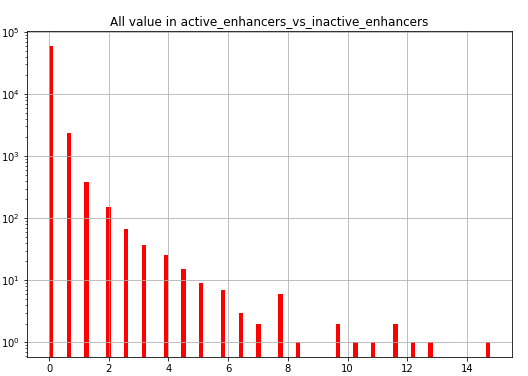
\includegraphics[width=\textwidth]{image/All_ae_vs_ie.PNG}
            \caption{All TPM value \acrshort{AE-IE} task.}
            \label{fig:All_ae_vs_ie}
        \end{minipage}
        \begin{minipage}[t]{.8\textwidth}
            \centering
            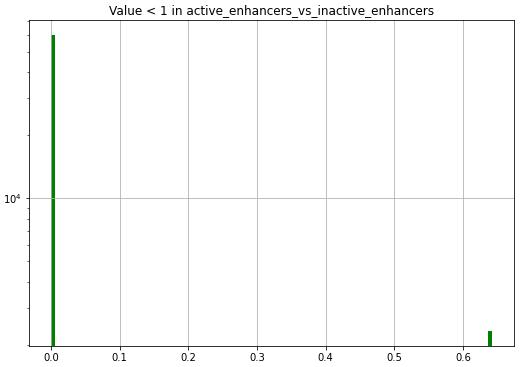
\includegraphics[width=\textwidth]{image/Restrict_ae_vs_ie.PNG}
            \caption{\acrshort{AE-IE} TPM value in range 0-1.}
            \label{fig:Restrict_ae_vs_ie}
        \end{minipage}
    \end{center}
\end{figure}

\noindent\newline
By displaying the histogram shown in the Figure \ref{fig:Restrict_ae_vs_ie}, and the red boxes of row 3 in Table \ref{tab:Threshold_Task}, it's possible identify graphically and numerically that a threshold $< 0.75$ can be used for the task of the active enhancers vs inactive enhancers. Any value above $< 0.75$ would only increase the offset between positive and negative values. For \acrshort{AE-IE} task, the value $0$ identified by the green row in the Table \ref{tab:Threshold_Task} has been chosen as the threshold.

\begin{figure}[!ht]
    \begin{center}
        \begin{minipage}[t]{.8\textwidth}
            \centering
            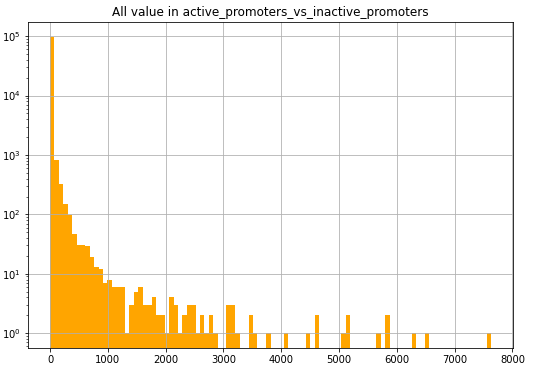
\includegraphics[width=\textwidth]{image/All_ap_vs_ip.PNG}
            \caption{All TPM value \acrshort{AP-IP} task.}
            \label{fig:All_ap_vs_ip}
        \end{minipage}
        \begin{minipage}[t]{.8\textwidth}
            \centering
            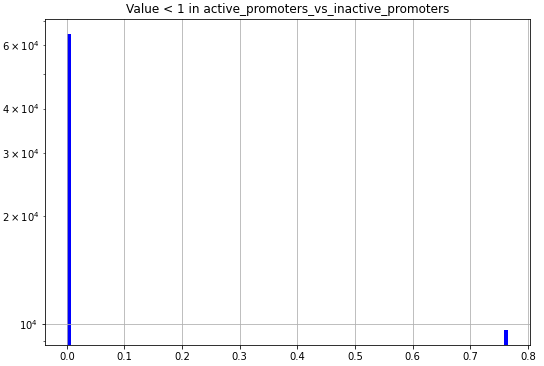
\includegraphics[width=\textwidth]{image/Restrict_ap_vs_ip.PNG}
            \caption{\acrshort{AP-IP} TPM value in range 0-1.}
            \label{fig:Restrict_ap_vs_ip}
        \end{minipage}
    \end{center}
\end{figure}

\noindent\newline
By displaying the histogram shown in the Figure \ref{fig:Restrict_ap_vs_ip}, and the red boxes of row 9 in Table \ref{tab:Threshold_Task}, it's possible identify graphically and numerically that the reason for the lack variation of the average with the first threshold values chosen (0, 0.25, 0.5). In fact, it emerges from the graphic representation that for values greater than 0 there is a real gap. For \acrshort{AP-IP} task, the value $1$ identified by the blue row in the Table \ref{tab:Threshold_Task} has been chosen as the threshold.

\noindent\newline
In some real world datasets, and especially biological and medical datasets, we often encounter a strong imbalance between classes. The more unbalanced the classes, the harder it becomes for us to create good models to predict them. It's therefore important to know immediately if the classes are more or less balanced or we are in a highly unbalanced scenario. For this reason after this binary exploration, useful for identifying the thresholds, we can see in Figure \ref{fig:Class_Balance} the unbalancing of the classes for the two tasks.

\begin{figure}
    \centering
    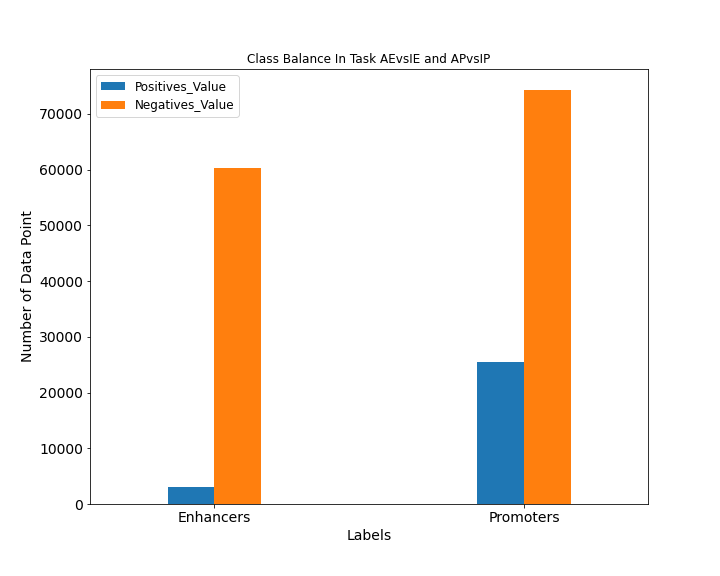
\includegraphics[width=12cm]{image/Class_Balance_AEvsIE_and_APvsIP.png}
    \caption{Class Balance Between \acrshort{AE-IE} and \acrshort{AP-IP} Task.}
    \label{fig:Class_Balance}
\end{figure}

\begin{table}
\begin{center}
\begin{tabular}{ | c | c | c |}
\hline
Region & Positives Value & Negatives Value \\
\hline
Enhancers & 3038 & 60247 \\
\hline
Promoters & 25559 & 74322 \\
\hline
\end{tabular}
\caption{\label{tab:Imbalance_Numerical} Numerical data between positives and negatives samples.}
\end{center}
\end{table}

\subsection{Data pre-processing}
\label{sec:Data_Pre_Processing}
To use sequence data, categorical values need to be converted to a BED\footnote{\url{https://www.ensembl.org/info/website/upload/bed.html}} format. This is done through one-hot encoding,
using the keras\_bed\_sequence python package, which allows us to obtain a matrix representation starting from the sequence of the human genome (Example AAATGG...TCA...TCCAT).
Finally, after data retrieval and generate sequence data, we can move on data elaboration section.

\subsection{Data Elaboration}
\label{sec:Data_Elaboration}
Data preprocessing is an important step in machine learning projects. Specifically it refer to manipulation or dropping of data before it's used in order to ensure or enhance performance. The steps performed are:
\begin{enumerate}
    \item Rate between features and samples
    \item Nan detection and imputation
    \item Constant detection
    \item Drop Constant features
    \item Feature Scaling
    \item Feature Correlations and Distributions
    \item Feature Selection
\end{enumerate}

\subsubsection{Rate between features and samples}
\label{subsec:Rate_between_features_and_samples}
In some datasets, there are more features than samples. This can introduce problems such as a particularly strong overfitting of the model. For this reason it's good practice to check if the datasets have a rate between features and samples greater than one. In a study case that has been analyzed, and in the datasets in use, it can be seen from the Table that the rate is well above 1.

\begin{table}[!ht]
\begin{center}
\begin{tabular}{ | c | c | c | c |}
\hline
Region & Total Sample & Features & Features Rate \\
\hline
Enhancers & 63285 & 58 & \textcolor{red}{1091.12} \\
\hline
Promoters & 99881 & 58 & \textcolor{red}{1722.09} \\
\hline
\end{tabular}
\caption{\label{tab:features_samples_rate} Rate Between Features and Samples.}
\end{center}
\end{table}

\subsubsection{Nan detection and imputation}
\label{subsec:Nan_detection_and_imputation}
From a theoretical and practical point of view, the presence of NaN (Not a Number) values or missing values within a dataset is a problem. Theoretically these values cannot be interpreted, while from a practical point of view their presence can cause errors during the execution of the algorithms, or provide incorrect data when evaluating some metrics. In order to deal with them, a k-Nearest Neighbors (k is a parameter that can be varied) Imputer\footnote{\url{https://scikit-learn.org/stable/modules/generated/sklearn.impute.KNNImputer.html}} is used to impute the missing values. The latter used by default, a euclidean distance metric that supports missing values is used to find the nearest neighbors. Each sample’s missing values are imputed using the mean value from nearest 5 (Five is a default value) neighbors found in the training set.

\subsubsection{Constant Detection}
\label{subsec:Constant_Detection}
We can also insert within this section the task of detecting constant features inside a dataset. Surely their presence doesn't involve important problems like those that are instead introduced by missing values, but their search and elimination is also part of the data cleaning. In general, it's not very common to find constant features inside the datasets, and most of the time it's a symptom that indicates that something is wrong in the data itself, but by not providing added value to each sample they can be eliminated. In the dataset in use for this project and for the specific cell line, no constant features to be eliminated have been identified.

\subsection{Feature Scaling}
\label{sec:Feature_Scaling}
Feature scaling, or normalization, is a method used to achieve comparable features across their range of values. In general, in this type of situations where the features aren't normalized, the network and the models in general should be able to adapt by changing the weights of the network, but what we want is to obtain weights as optimized as possible to better manage the label in exit and not to self-normalize the weights of the network, making learning more difficult and longer, among other things.
\noindent
In linear classifiers, for example, if a characteristic takes on high values, it's importance is greater in forecasting than another characteristic with lower values. We want to avoid this and other common problems with unsized features.
\noindent
To obviate the above, a Robust Scaler\footnote{\url{https://scikit-learn.org/stable/modules/generated/sklearn.preprocessing.RobustScaler.html}} is used, which as the name suggests is a robust tool, especially towards the outliers (which are the ones we want to eliminate) which allows us to normalize the data by subtracting the median and dividing by the standard deviation within an interquartile\footnote{\url{https://it.wikipedia.org/wiki/Scarto_interquartile}} range between 0.25 and 0.75. Therefore, given a Gaussian distribution, we will remove the initial e part and the tail of the distribution, in order to avoid bringing values that tend towards infinity into the dataset.
\noindent
It should also be remembered that this normalization problem has a very high impact in networks, or in any case in models that include layers where the sum of the various features is performed. Unlike in models such as decision trees, the problem doesn't exist.

\subsection{Data Correlations and Distributions}
\label{sec:Data_Correlations_and_Distributions}

\subsubsection{Feature Correlation}
\label{sec:Feature_Correlations}
Another parameter that we can evaluate is that of correlation. The latter can be applied with respect to output labels or between features. What are we going to determine with the correlation? Correlation is a specific analysis that measures the strength of the association between two variables and the direction of the relationship. In terms of the strength of the relationship, the value of the correlation coefficient varies between +1 and -1. When it's close to 1 it means that there is a strong positive correlation whereas when the coefficient is close to -1, it means that there is a strong negative correlation. Finally, coefficients close to 0 mean that there is non linear correlation, but this does not mean that there is no correlation. For this reason, in addition to the application of the Pearson\footnote{\url{https://it.wikipedia.org/wiki/Indice_di_correlazione_di_Pearson}} and Spearman\footnote{\url{https://it.wikipedia.org/wiki/Coefficiente_di_correlazione_per_ranghi_di_Spearman}} indices, the \acrshort{MIC}\footnote{\url{https://en.wikipedia.org/wiki/Maximal_information_coefficient}} (maximum coefficient of information) which is a measure based on non-parametric statistics was used. It helps us determine the strength of the linear or non-linear association between two variables X and Y. Given a certain correlation threshold, we will then determine what are the features not correlated with the output labels, and if present they can also be eliminated.

\begin{figure}[!ht]
    \centering
    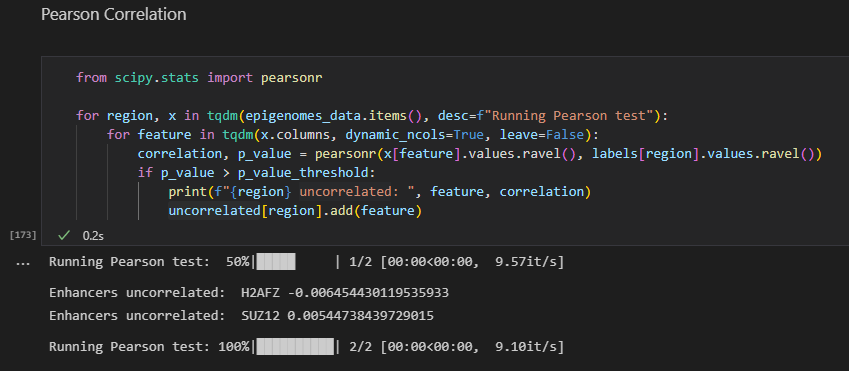
\includegraphics[width=12cm]{image/Pearson.PNG}
    \caption{Pearson Correlation.}
    \label{fig:Pearson}
\end{figure}

\noindent
Once the correlation steps with the output have been completed, it can be seen on Figure \ref{fig:MIC} that the features identified by the \textbf{H2AFZ}, \textbf{UZ12} labels are not related to the output labels and therefore can be eliminated. Obviously their presence does not involve problems during the training of the models, but when we have a very high number of features, their elimination can greatly facilitate the training phase.

\begin{figure}[!ht]
    \centering
    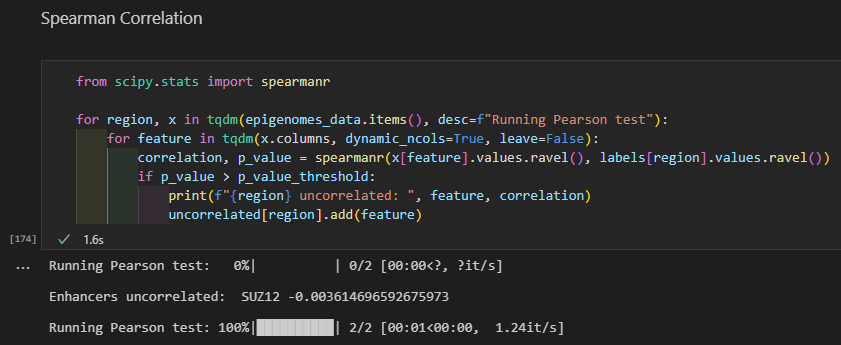
\includegraphics[width=12cm]{image/Spearman.PNG}
    \caption{Spearman Correlation.}
    \label{fig:Spearman}
\end{figure}

\begin{figure}[!ht]
    \centering
    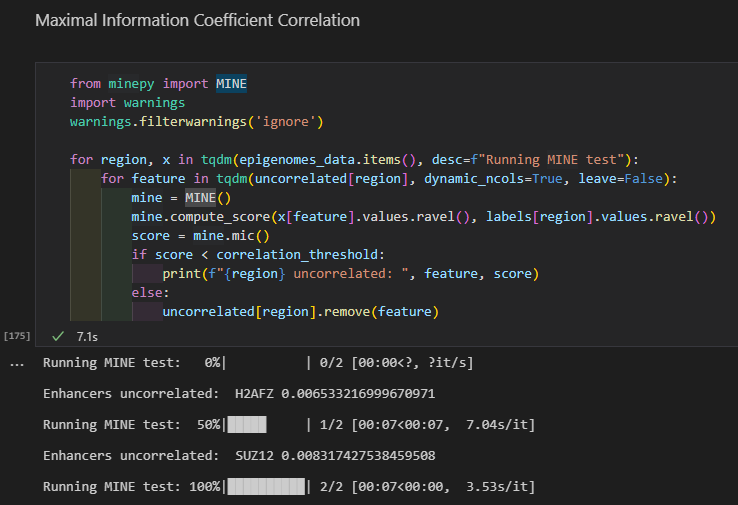
\includegraphics[width=12cm]{image/MIC.PNG}
    \caption{Maximal Information Coefficient Correlation.}
    \label{fig:MIC}
\end{figure}

\noindent
The next step was to identify and drop features that have extremely high Pearson correlation values (greater than 0.90 or even than 0.99) with each other. These features often don't add meaningful information when removed. If we have to choose to remove a feature, we will remove the one with lower entropy. In information theory, the entropy\footnote{\url{https://it.wikipedia.org/wiki/Entropia_(teoria_dell\%27informazione)}} of a message source is the average information contained in each sent message. The information contained in a message is the greater the less likely it was. A foregone message, which has a high probability of being emitted by the source, contains little information, while an unexpected, unlikely message contains a large amount of information.

\begin{figure}[!ht]
    \centering
    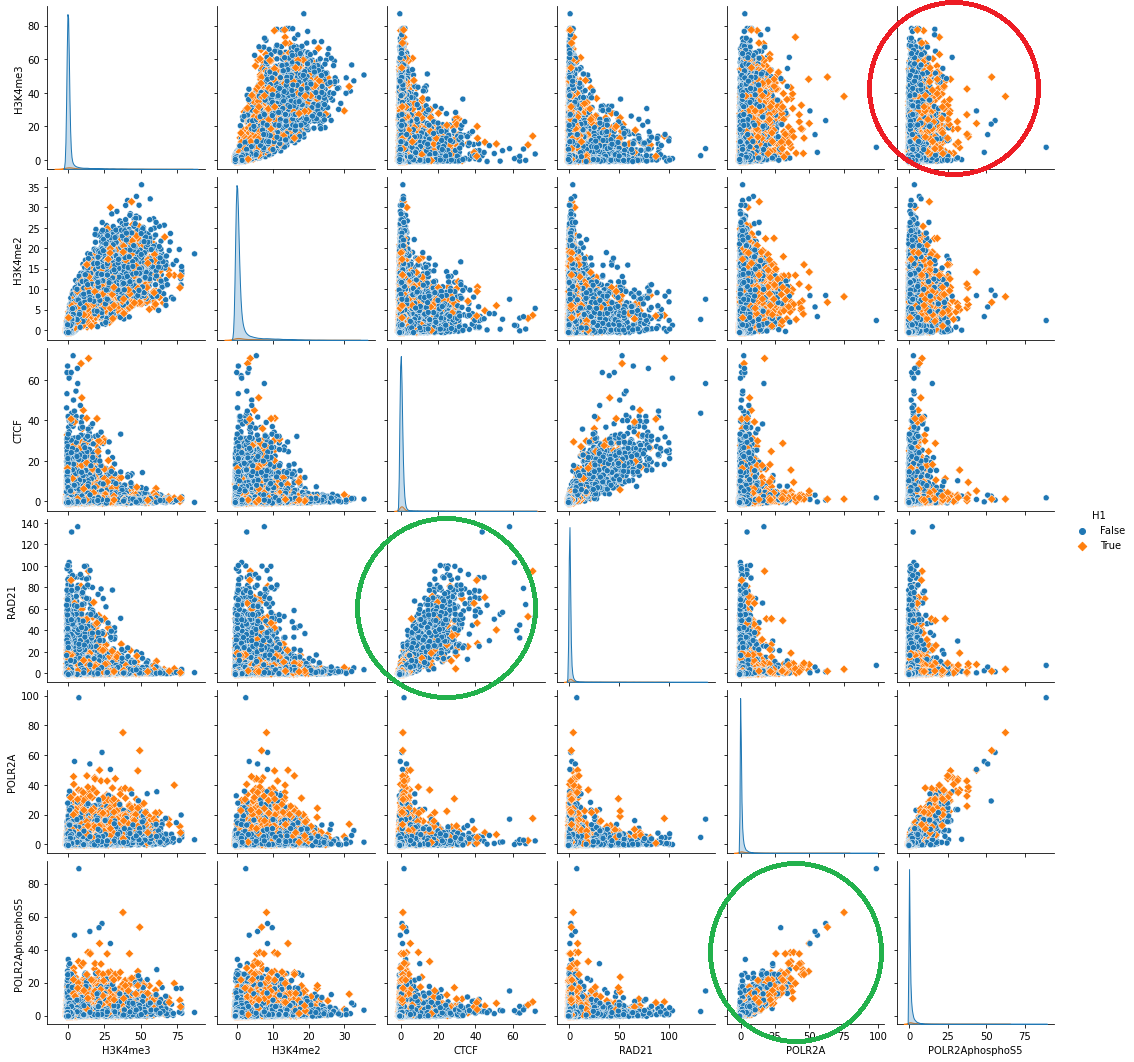
\includegraphics[width=7cm]{image/Features_Correlation_Enhancers_Box.PNG}
    \caption{Most Correlated Features In Enhancers Region.}
    \label{fig:Features_Correlation_Enhancers}
\end{figure}

\noindent
We show the top five (where possible) most correlated features in promoters and enhancers in Figure \ref{fig:Features_Correlation_Enhancers} and Figure \ref{fig:Features_Correlation_Promoters} respectively. Blue square they indicate the samples of the inactive regions, while the orange diamonds indicate the active regions. Since no features highly correlated with statistical significance are found, we will keep all the features.

\begin{figure}[!ht]
    \centering
    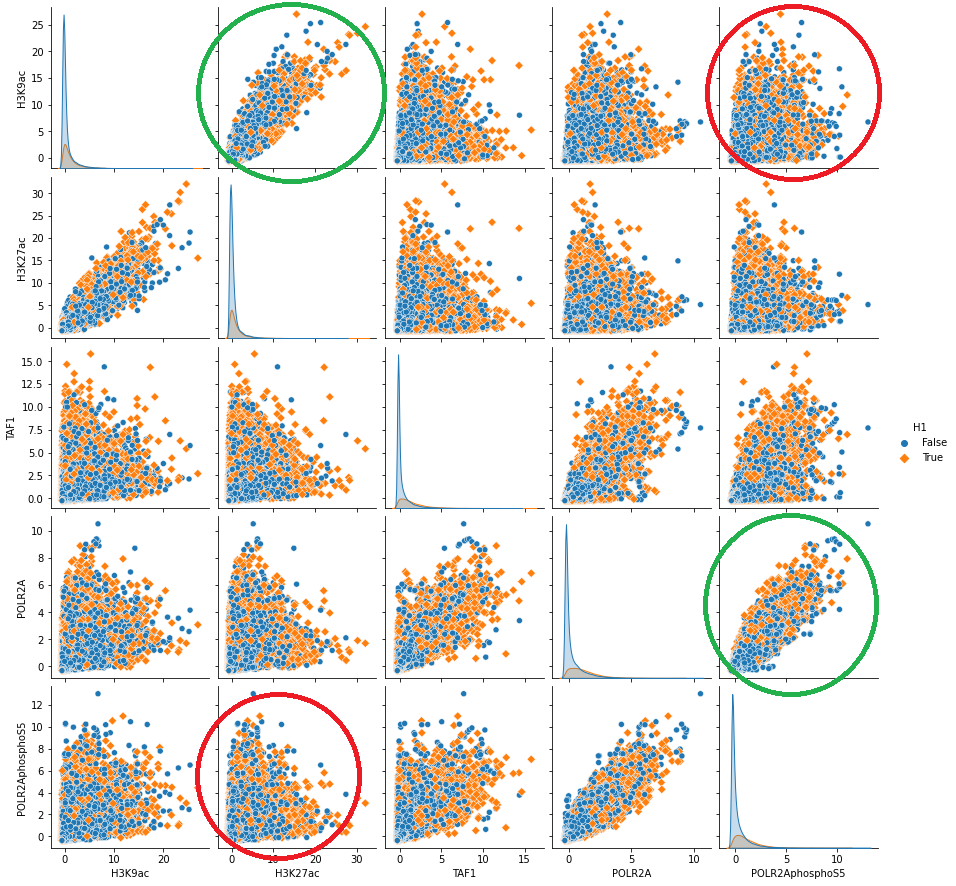
\includegraphics[width=7cm]{image/Features_Correlation_Promoters_Box.PNG}
    \caption{Most Correlated Features In Promoters Region.}
    \label{fig:Features_Correlation_Promoters}
\end{figure}

\noindent
This plot allows us to graphically identify the most correlated features (green circles), which are those that are positioned on the diagonal or antidiagonal, vice versa all the others, that in general the samples tend to accumulate towards one of the two axes, are considered unrelated (red circles). In the main diagonal is possible to see the distribution of a single feature. In general for the inactive value there are a lot of sample most close to zero, while for the active regions we have a small Gaussian distribution.

\begin{figure}[!ht]
    \centering
    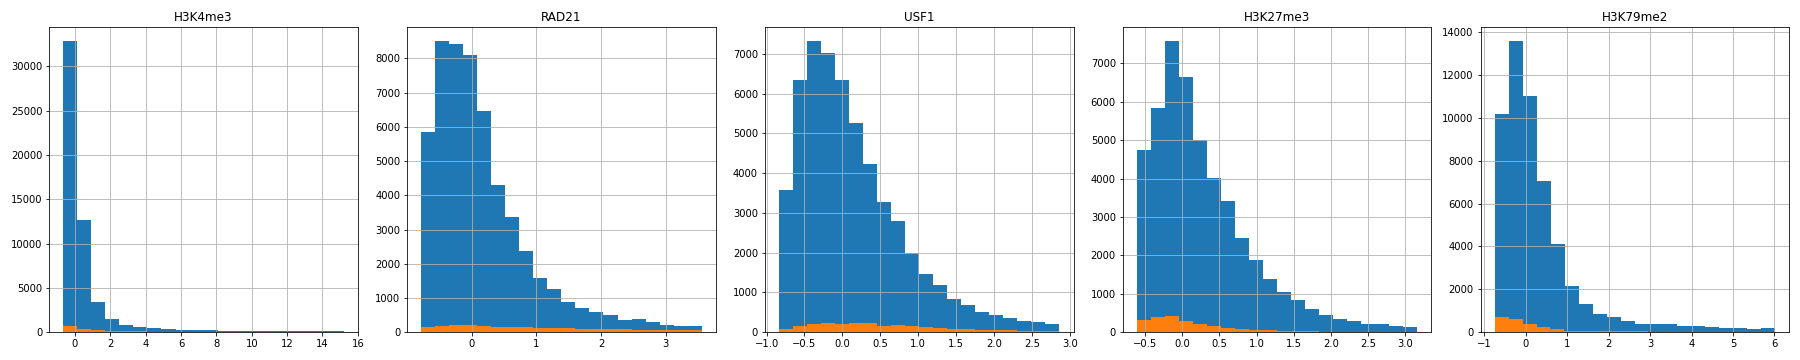
\includegraphics[width=12cm]{image/Top_5_Features_Distribution_Enhancers.PNG}
    \caption{Top 5 Features Distribution In Enhancers Region.}
    \label{fig:Top_Features_Enhancers}
\end{figure}

\begin{figure}[!ht]
    \centering
    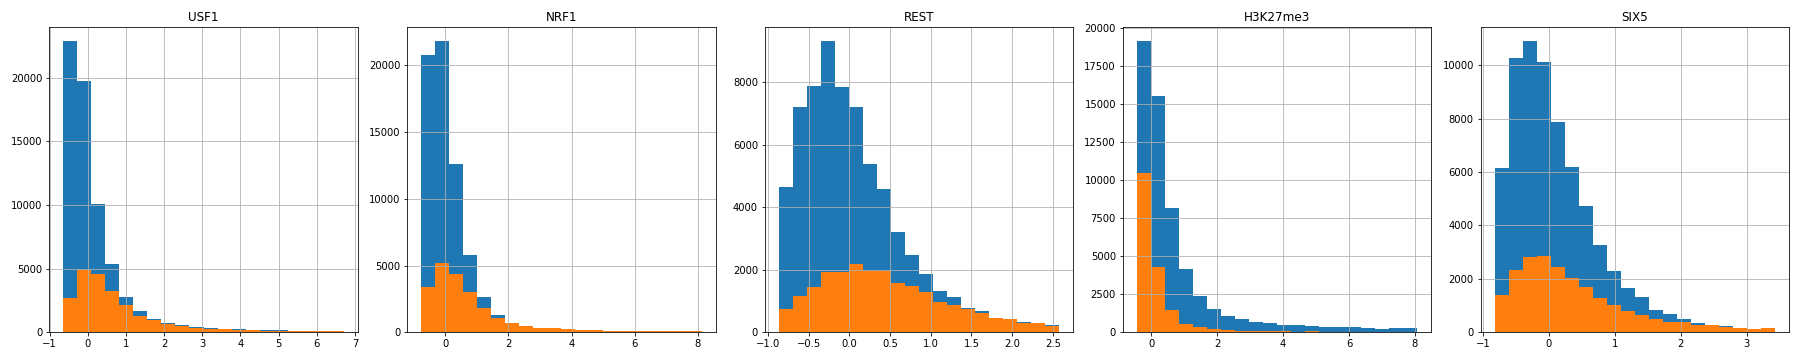
\includegraphics[width=12cm]{image/Top_5_Features_Distribution_Promoters.PNG}
    \caption{Top 5 Features Distribution In Promoters Region.}
    \label{fig:Top_Features_Promoters}
\end{figure}

\subsubsection{Feature Distributions}
\label{sec:Feature_Distributions}
\noindent
Also, we want to show the distributions of the epigenomic features. Since there are 58 features, and we cannot show all the distributions, we select the top 5 most different features (5 for promoters and 5 for enhancers), using the pairwise euclidean distance between the features, and represent their distributions using histograms on a log scale. Figure \ref{fig:Top_Features_Enhancers} shows the top 5 most different features for promoters and Figure \ref{fig:Top_Features_Promoters} shows the top 5 most different features for enhancers. Analyzing the distribution of features is a way to also understand how separable the classes in question are. Furthermore, given the alignment between them, it’s possible to determine which features are particularly informative and relevant in the training phase and which are not.

\subsection{Feature Selection}
Feature selection is one of the core concepts in machine learning which hugely impacts the performance of your model. The data features that you use to train your machine learning models have a huge influence on the performance you can achieve. Both correlation with output and correlation between features can be used for the selection of features, but there are numerous techniques for running feature selection. In this project we will use Boruta\footnote{\url{https://www.jstatsoft.org/article/view/v036i11}} using the python package Boruta\_py\footnote{\url{https://github.com/scikit-learn-contrib/boruta_py}}. Boruta is based on statistical tests performed on the performances calculated through a random forest classifier. The random forest gives the importance of each characteristic, replacing it with a random set of values. Comparing the importance of the feature between the feature itself and the set of values that replaced it, if the result is the same it means that the feature in question is not useful at all. It's a very expensive technique, which is why during the realization of the project it was performed with a maximum number of iterations equal to 30.

\subsection{Data Visualization}
\label{sec:data_visualization}
In this section, we explore two techniques used for data transformation and visualization. Specifically, most of the datasets used in bioinformatics, but in machine learning in general, have a number of features that far exceed the 3 dimensions of space, with which it's possible to perform the projection inside a cube, otherwise we would fall back into hyperspace. For this reason these techniques allow us to reduce the dimensionality while preserving the maximum amount of information.
\begin{itemize}
    \item PCA: It's a technique aimed at deriving, starting from a set of correlated numerical variables, a smaller set of “artificial” orthogonal variables. The reduced set of linear orthogonal projections (known as "principal components" or "principal components", "PC") is obtained by linearly combining the original variables in an appropriate manner.
    \item t-SNE: t-SNE is a statistical method for visualizing high-dimensional data by giving each data point a location in a two or three dimensional map. It's a nonlinear dimensionality reduction technique well-suited for embedding high-dimensional data for visualization in a low-dimensional space of two or three dimensions. Specifically, it models each high-dimensional object by a two- or three-dimensional point in such a way that similar objects are modeled by nearby points and dissimilar objects are modeled by distant points with high probability.\cite{enwiki:1040619466}
\end{itemize}
    
\begin{figure}
    \centering
    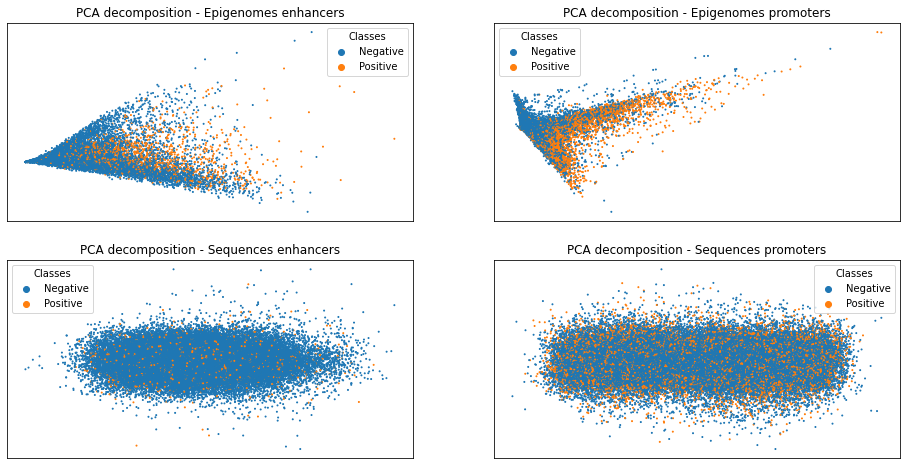
\includegraphics[width=12cm]{image/PCA_2.png}
    \caption{PCA Applied To Epigenomic And Sequence Data.}
    \label{fig:PCA}
\end{figure}

\begin{figure}
    \centering
    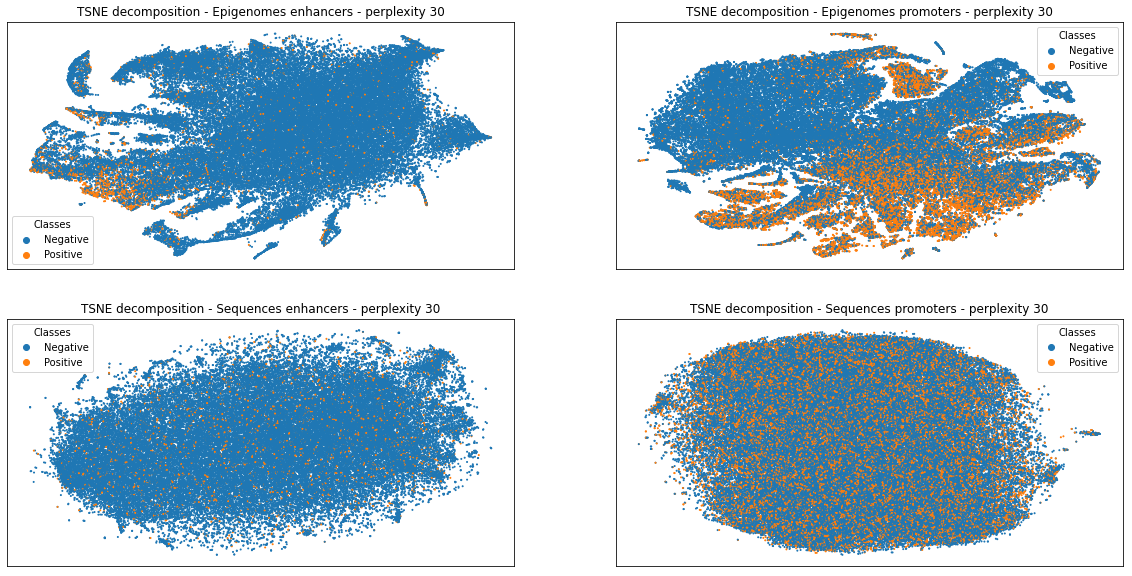
\includegraphics[width=12cm]{image/+30_TSNE.png}
    \caption{t-SNE With 30 Perplexity}
    \label{fig:30_Perplexity}
\end{figure}

\begin{figure}
    \centering
    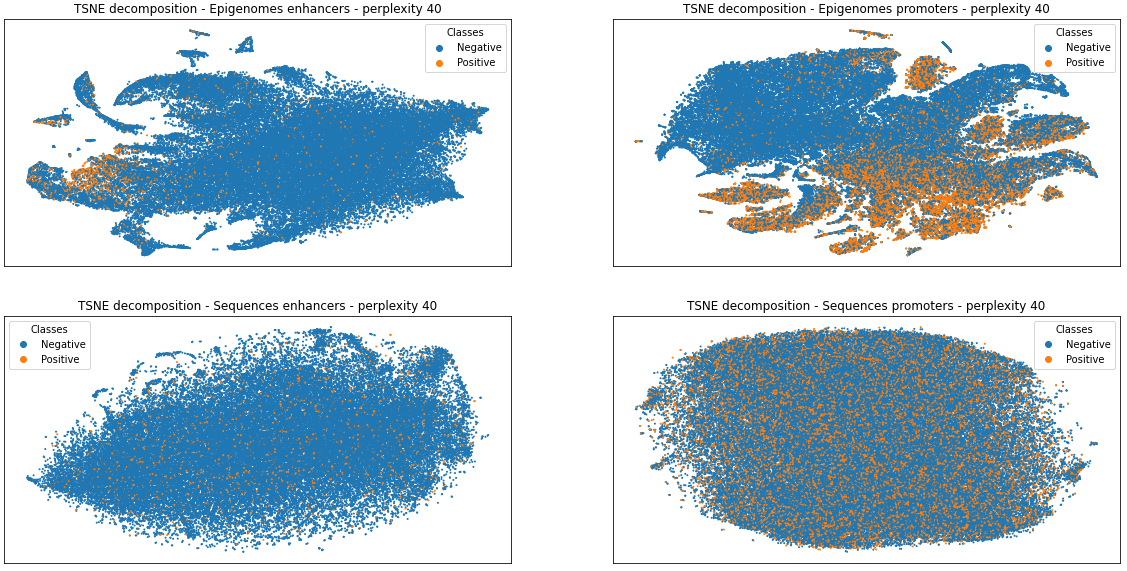
\includegraphics[width=12cm]{image/+40_TSNE.png}
    \caption{t-SNE With 40 Perplexity}
    \label{fig:40_Perplexity}
\end{figure}

\begin{figure}
    \centering
    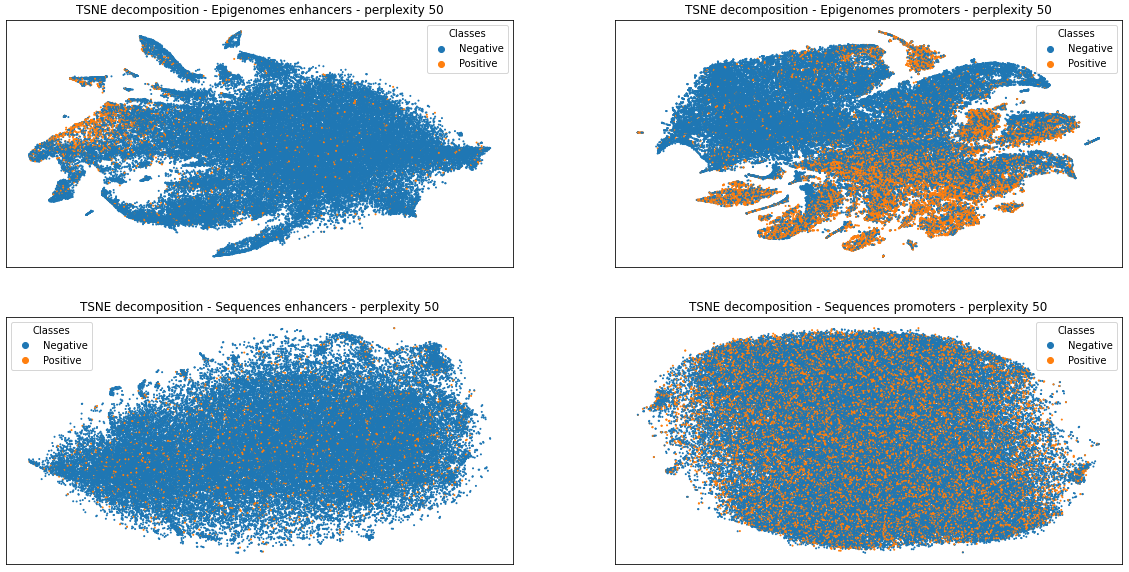
\includegraphics[width=12cm]{image/+50_TSNE.png}
    \caption{t-SNE With 50 Perplexity}
    \label{fig:50_Perplexity}
\end{figure}

\begin{figure}
    \centering
    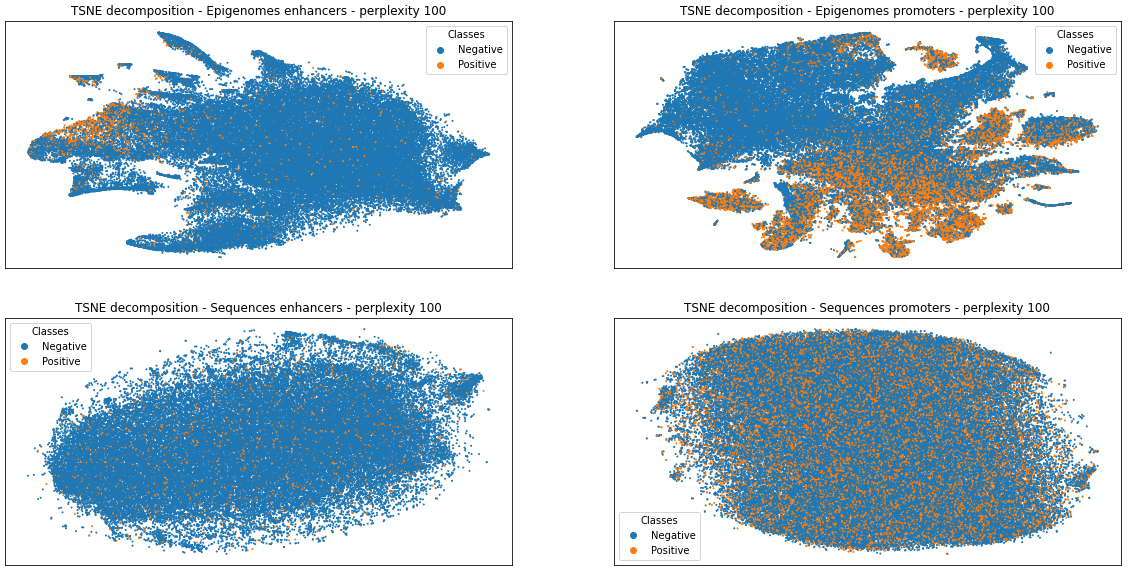
\includegraphics[width=12cm]{image/+100_TSNE.png}
    \caption{t-SNE With 100 Perplexity}
    \label{fig:100_Perplexity}
\end{figure}

\begin{figure}
    \centering
    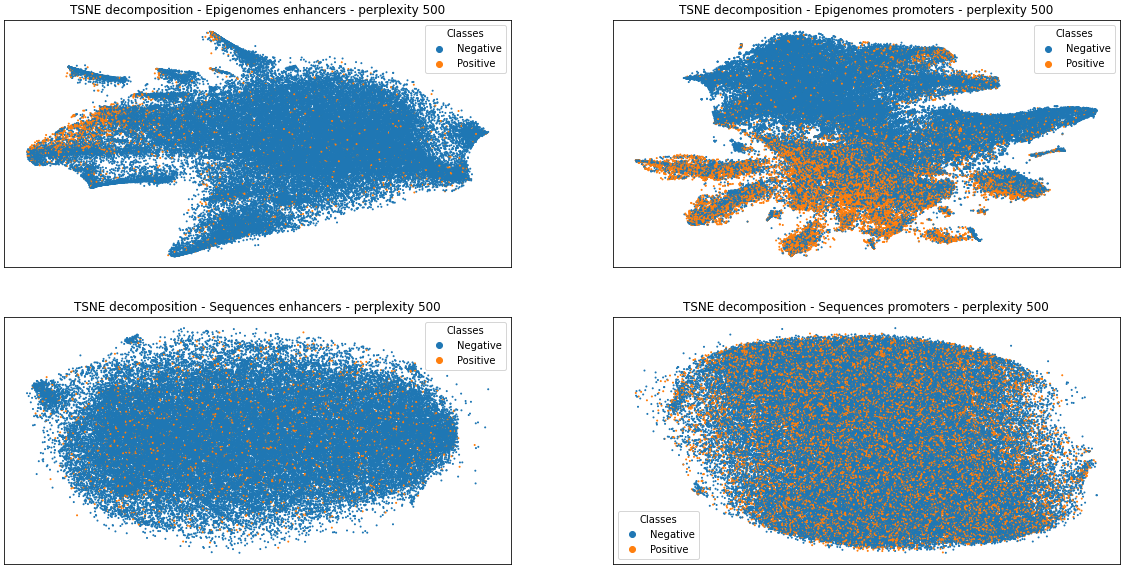
\includegraphics[width=12cm]{image/+500_TSNE.png}
    \caption{t-SNE With 500 Perplexity}
    \label{fig:500_Perplexity}
\end{figure}

\begin{figure}
    \centering
    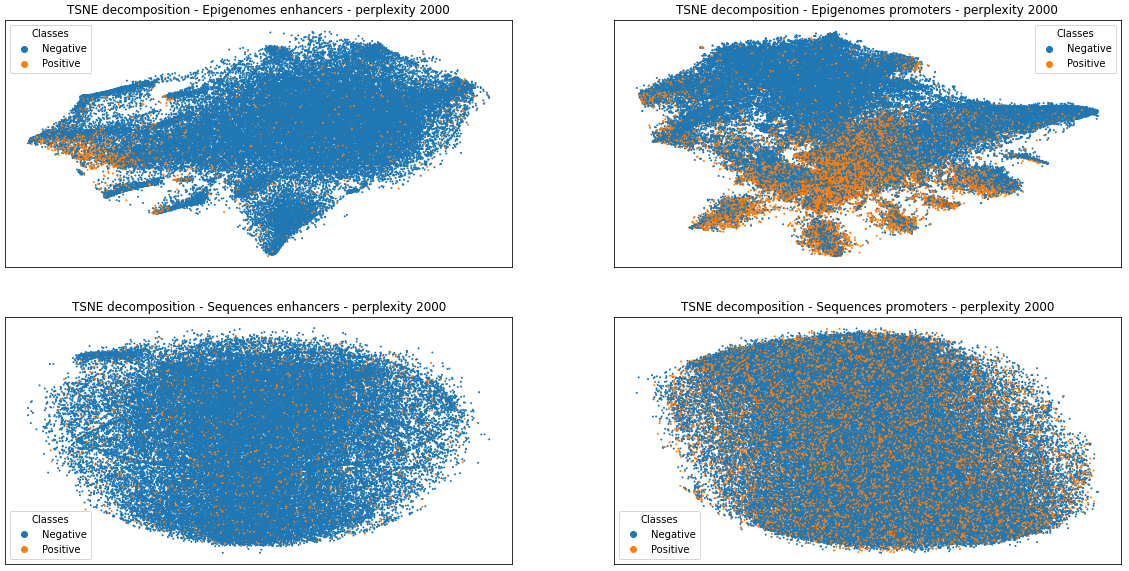
\includegraphics[width=12cm]{image/+2000_TSNE.png}
    \caption{t-SNE With 2000 Perplexity}
    \label{fig:2000_Perplexity}
\end{figure}

\noindent
In Figure \ref{fig:30_Perplexity}, \ref{fig:40_Perplexity}, \ref{fig:50_Perplexity}, \ref{fig:100_Perplexity}, \ref{fig:500_Perplexity}, \ref{fig:2000_Perplexity} shows the results of t-SNE applied to epigenomic and sequence data in both promoter and enhancer regions with different value of perplexity\footnote{\url{https://en.wikipedia.org/wiki/Perplexity}}, while in the Figure \ref{fig:PCA} the representation of the same data performed with the PCA algorithm with a number of components equal to 2.

\subsection{Holdouts}
\label{sec:Holdouts}
In order to evaluate the models we executed 10 holdouts, each of which, after shuffling the data, split the data sets in a training set that containing 80\% of the data and in a test set containing the remaining 20\% of the data. In doing so, we preserved the stratification of the classes in both the training and test sets. This subdivision approach into train data and test data is necessary to verify the generalization capacity of the trained model (train data) on unseen data (train data).

\subsection{Metrics}
\label{sec:Metrics}
Each model was evaluated according to mainly three metrics: area under the precision recall curve (AUPRC), area under the receiver operating characteristic curve (AUROC) and Accuracy (Loss plots are put in it only for give context in some point of results). Given the imbalance of the classes, the mean AUPRC over the test sets was considered the most informative predictor of the quality of the model.

\noindent
To gauge the existence of a statistical difference between models under comparison, we used the Wilcoxon signed-rank test. The Wilcoxon signed-rank \cite{wilcoxon} test tests the null hypothesis that two related paired samples come from the same distribution. In particular, it tests whether the distribution of the differences of two vector x - y is symmetric about zero for same sample. We considered a p-value lower than 0.01 (one error every 100) as a sensible threshold to claim that the compared models were statistically different.  

\section{Results}
\label{sec:Results}

\begin{enumerate}
    \item Once all the phases of the project were completed, we are created some graphs for help to understand the results obtained in a more concrete way. Specifically, it's possible to see a series of barplots based essentially on the metrics indicated in the section \ref{sec:Metrics}. For each task the results were grouped by model and if they had more or less used the feature selection.
    All the graphs referring to this section are those shown in the Figures \ref{fig:Loss_enhancers}, \ref{fig:Accuracy_enhancers}, \ref{fig:AUROC_enhancers}, \ref{fig:AUPRC_enhancers}, \ref{fig:Loss_promoters}, \ref{fig:Accuracy_promoters}, \ref{fig:AUROC_promoters}, \ref{fig:AUPRC_promoters}.
    
    \item In addition to the use of graphs only, an appropriate function based on the Wilcoxon test was used through which it's possible to determine in a formal way if one model was better than the other respect to some metrics. The results obtained are shown in the table \ref{tab:wilcoxon_result}.
    \newline
    \begin{table}[!ht]
    \begin{center}
    \begin{tabular}{  c | c | c | c | c }
    \hline
    Task & Model & Metrics & P\_Value & Result\\
    \hline
    Enhancers & BinaryClassificationFFNNV1 & AUPRC & 0.845 & \acrshort{ST}\\
    Enhancers & BinaryClassificationFFNNV1 & AUROC & 0.921 & \acrshort{ST}\\
    Enhancers & BinaryClassificationFFNNV1 & Accuracy & 0.275 & \acrshort{ST}\\
    \hline
    Enhancers & BinaryClassificationCNNV1 & AUPRC & 0.556 & \acrshort{ST}\\
    Enhancers & BinaryClassificationCNNV1 & AUROC & 0.625 & \acrshort{ST}\\
    Enhancers & BinaryClassificationCNNV1 & Accuracy & 1.0 & \acrshort{ST}\\
    \hline
    Enhancers & MMNNV1 & AUPRC & 0.921 & \acrshort{ST}\\
    Enhancers & MMNNV1 & AUROC & 0.695 & \acrshort{ST}\\
    Enhancers & MMNNV1 & Accuracy & 0.838 & \acrshort{ST}\\
    \hline
    Enhancers & BoostedMMNNV1 & AUPRC & 0.492 & \acrshort{ST}\\
    Enhancers & BoostedMMNNV1 & AUROC & 0.769 & \acrshort{ST}\\
    Enhancers & BoostedMMNNV1 & Accuracy & 0.695 & \acrshort{ST}\\
    \hline
    Promoters & BinaryClassificationFFNNV1 & AUPRC & 0.193 & \acrshort{ST}\\
    Promoters & BinaryClassificationFFNNV1 & AUROC & 0.019 & \acrshort{ST}\\
    Promoters & BinaryClassificationFFNNV1 & Accuracy & 0.037 & \acrshort{ST}\\
    \hline
    Promoters & BinaryClassificationCNNV1 & AUPRC & 0.130 & \acrshort{ST}\\
    Promoters & BinaryClassificationCNNV1 & AUROC & 0.130 & \acrshort{ST}\\
    Promoters & BinaryClassificationCNNV1 & Accuracy & 0.556 & \acrshort{ST}\\
    \hline
    Promoters & MMNNV1 & AUPRC & 0.431 & \acrshort{ST}\\
    Promoters & MMNNV1 & AUROC & 0.431 & \acrshort{ST}\\
    Promoters & MMNNV1 & Accuracy & 0.232 & \acrshort{ST}\\
    \hline
    Promoters & BoostedMMNNV1 & AUPRC & 0.921 & \acrshort{ST}\\
    Promoters & BoostedMMNNV1 & AUROC & 0.845 & \acrshort{ST}\\
    Promoters & BoostedMMNNV1 & Accuracy & 0.232 & \acrshort{ST}\\
    \hline
    \end{tabular}
    \caption{\label{tab:wilcoxon_result} Results For Wilcoxon Test Applied On Model With And Without Feature Selection.}
    \end{center}
    \end{table}
    
    \item Further graphical representation was used to point out once again, how the use of the boruta algorithm for this specific cell line, not only with a maximum number of iterations set to 30 it was not able to eliminate features, but that for the purpose of identifying an optimal value of AUPRC it was not supportive but added complexity and lengthened the execution times.
    
    \begin{figure}[!ht]
    \centering
    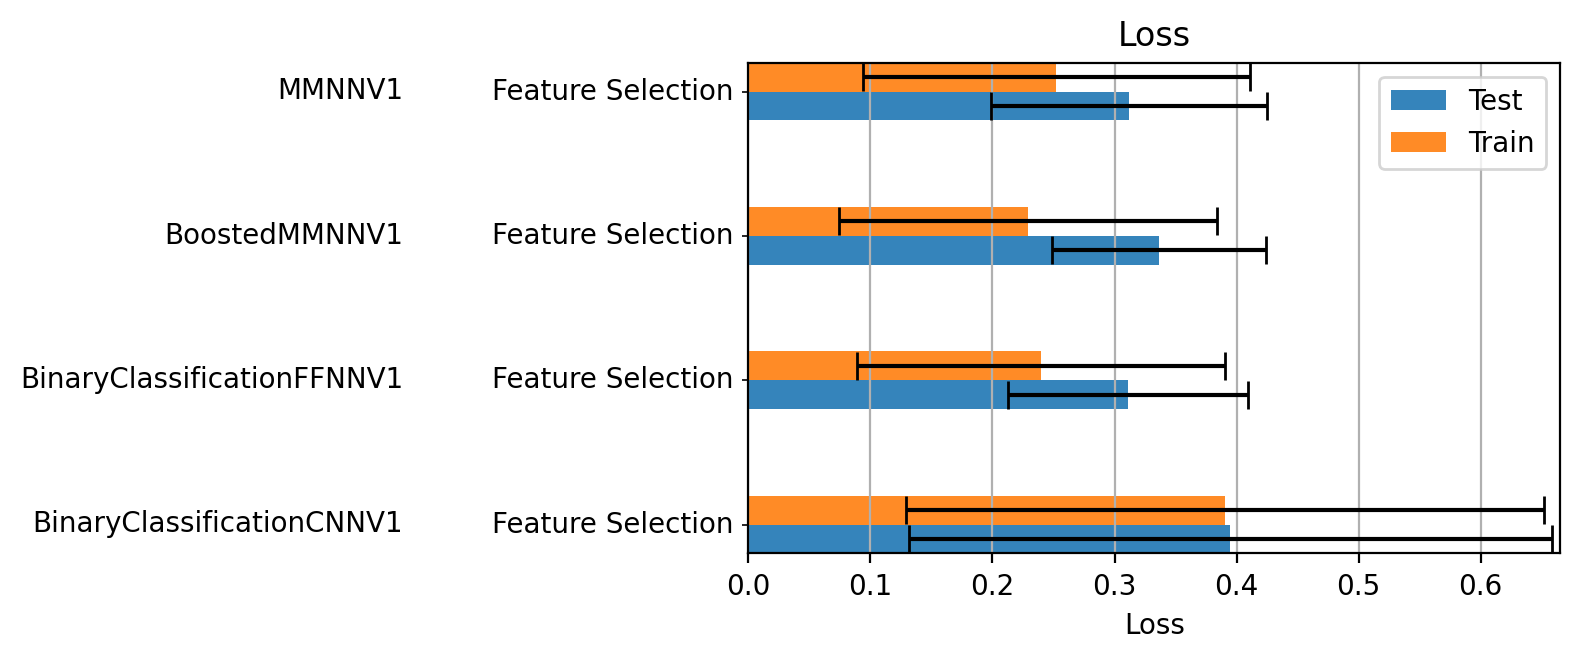
\includegraphics[width=11cm]{image/barplots/enhancers/Loss_enhancers.PNG}
    \caption{Loss Enhancers}
    \label{fig:Loss_enhancers}
    \end{figure}
    \begin{figure}[!ht]
        \centering
        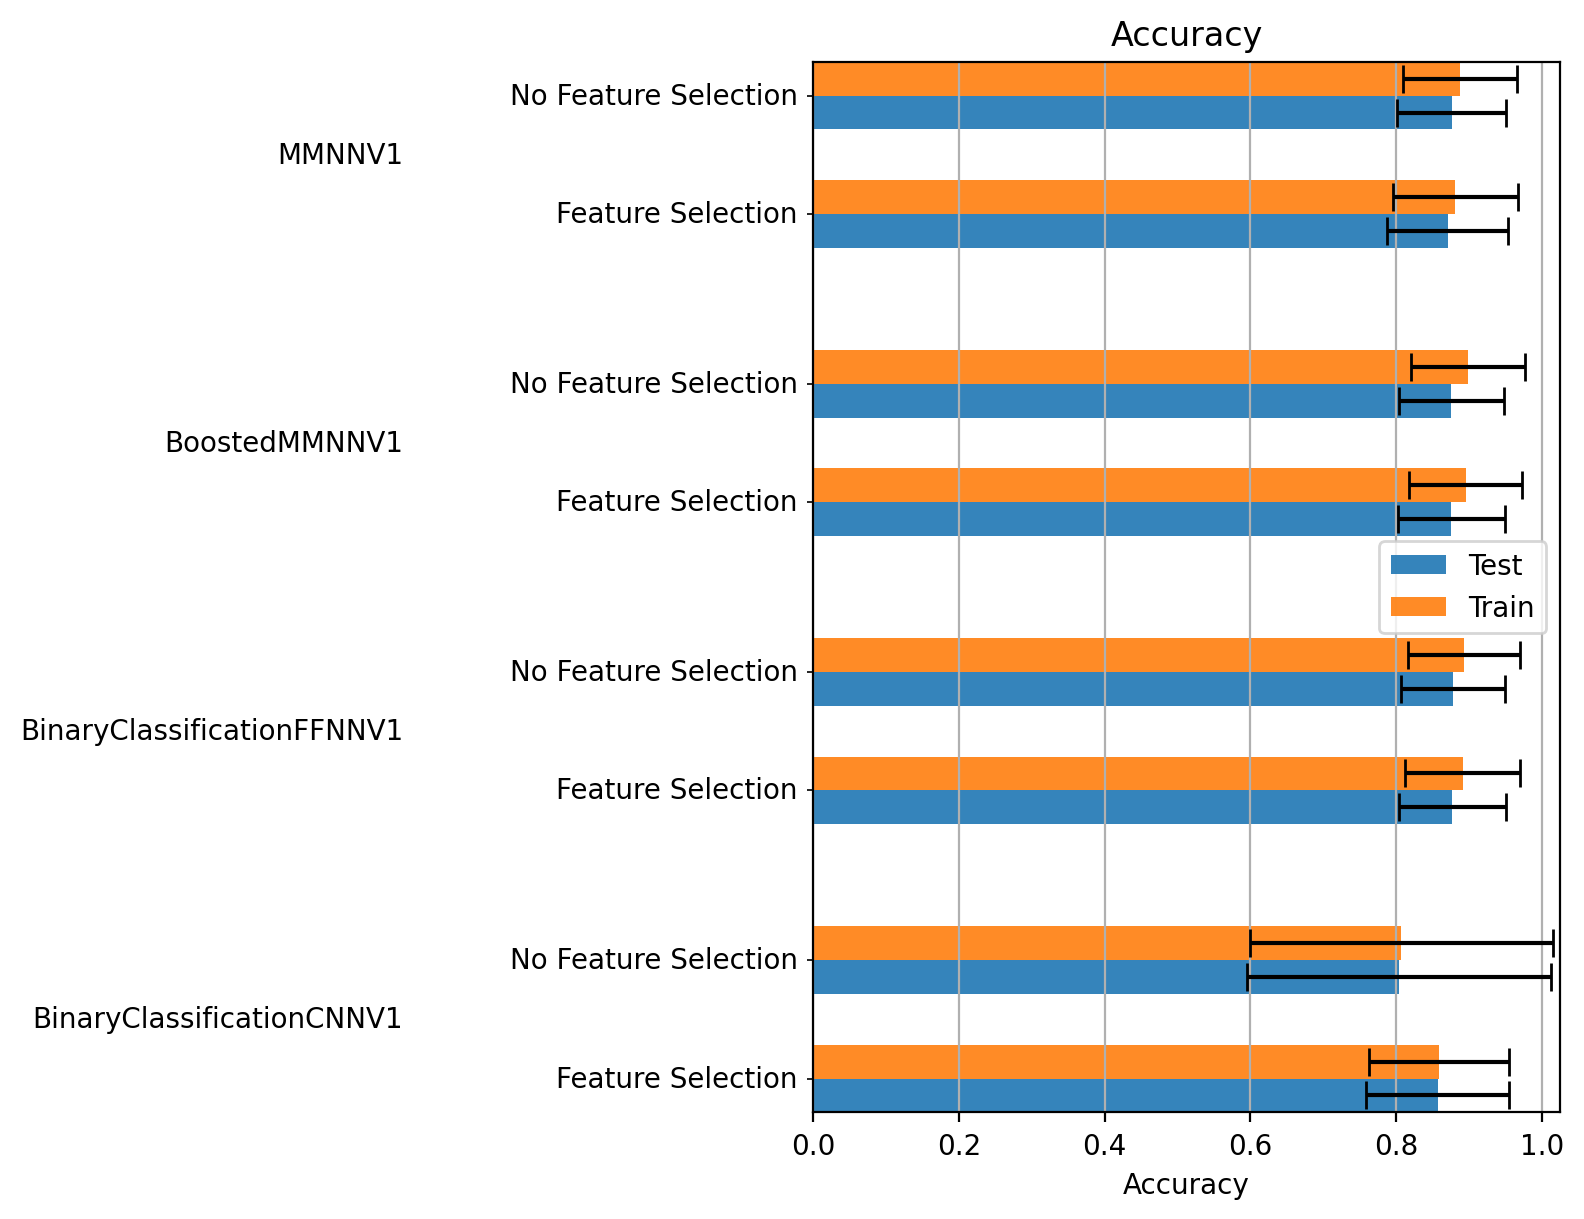
\includegraphics[width=11cm]{image/barplots/enhancers/Accuracy_enhancers.PNG}
        \caption{Accuracy Enhancers}
        \label{fig:Accuracy_enhancers}
    \end{figure}
    \begin{figure}[!ht]
        \centering
        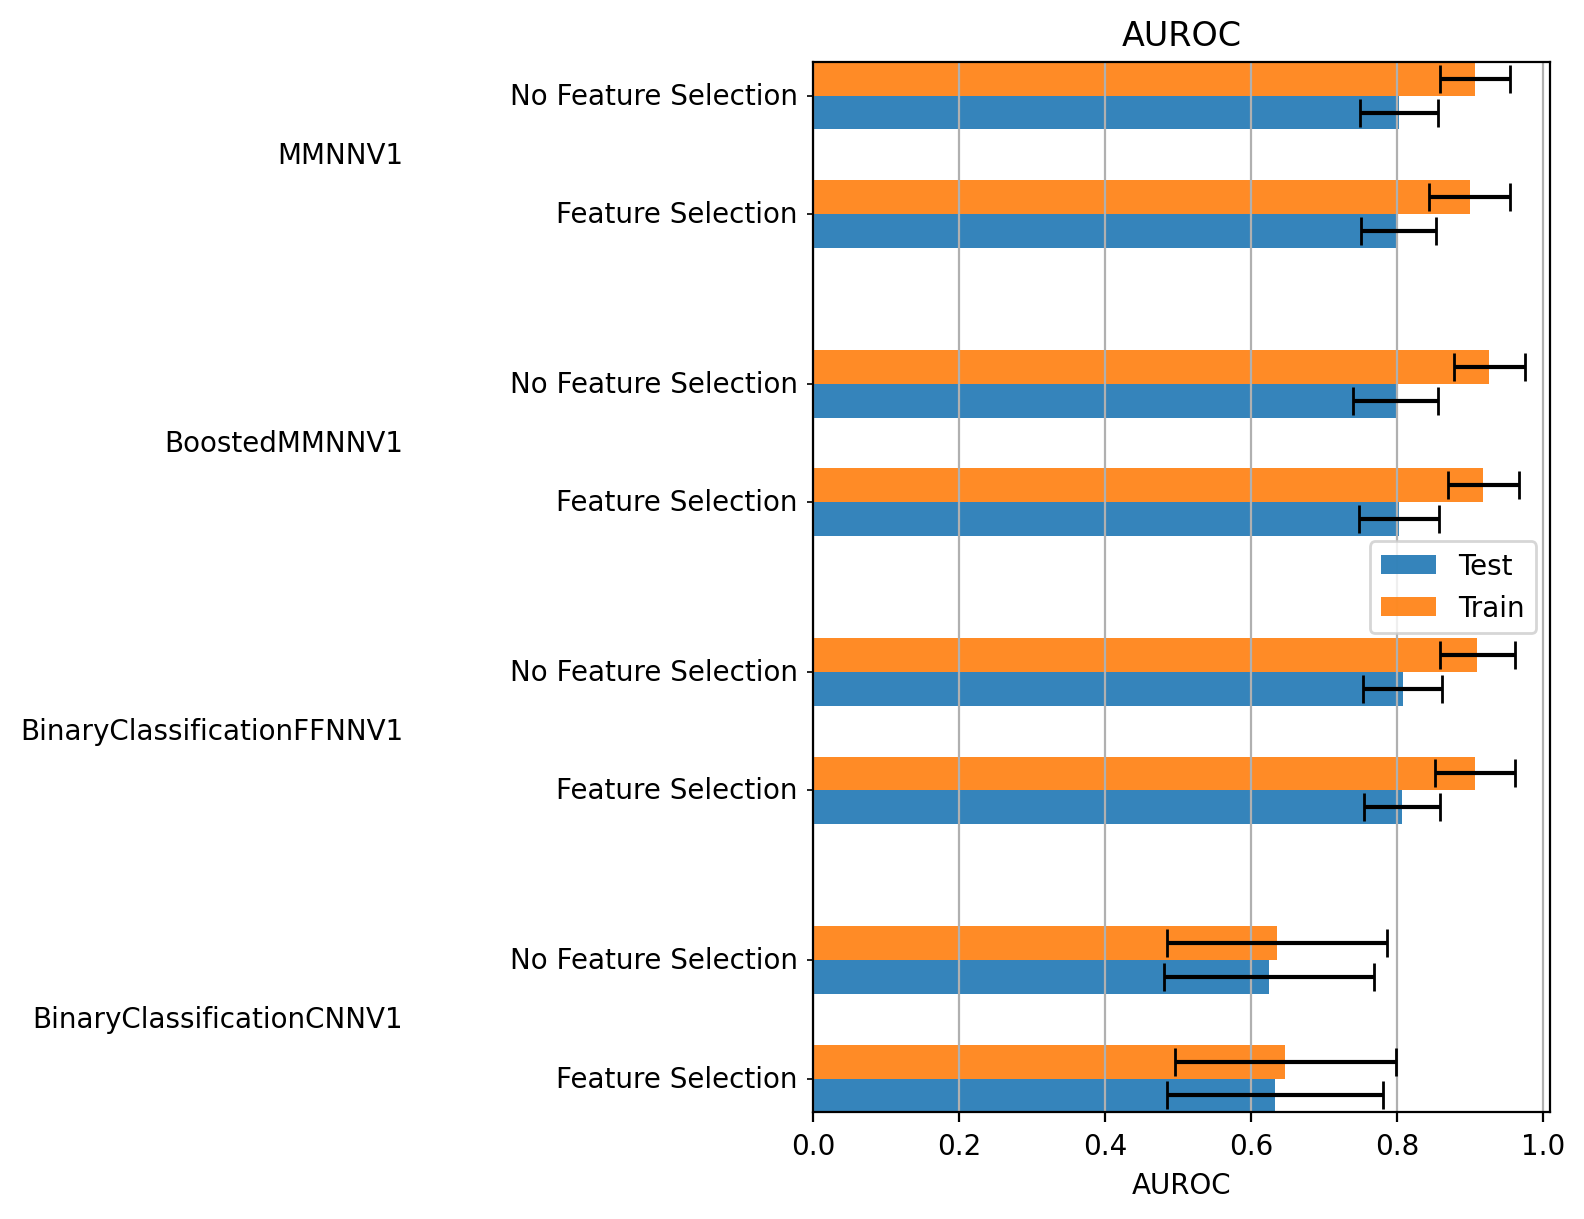
\includegraphics[width=11cm]{image/barplots/enhancers/AUROC_enhancers.PNG}
        \caption{AUROC Enhancers}
        \label{fig:AUROC_enhancers}
    \end{figure}
    \begin{figure}[!ht]
        \centering
        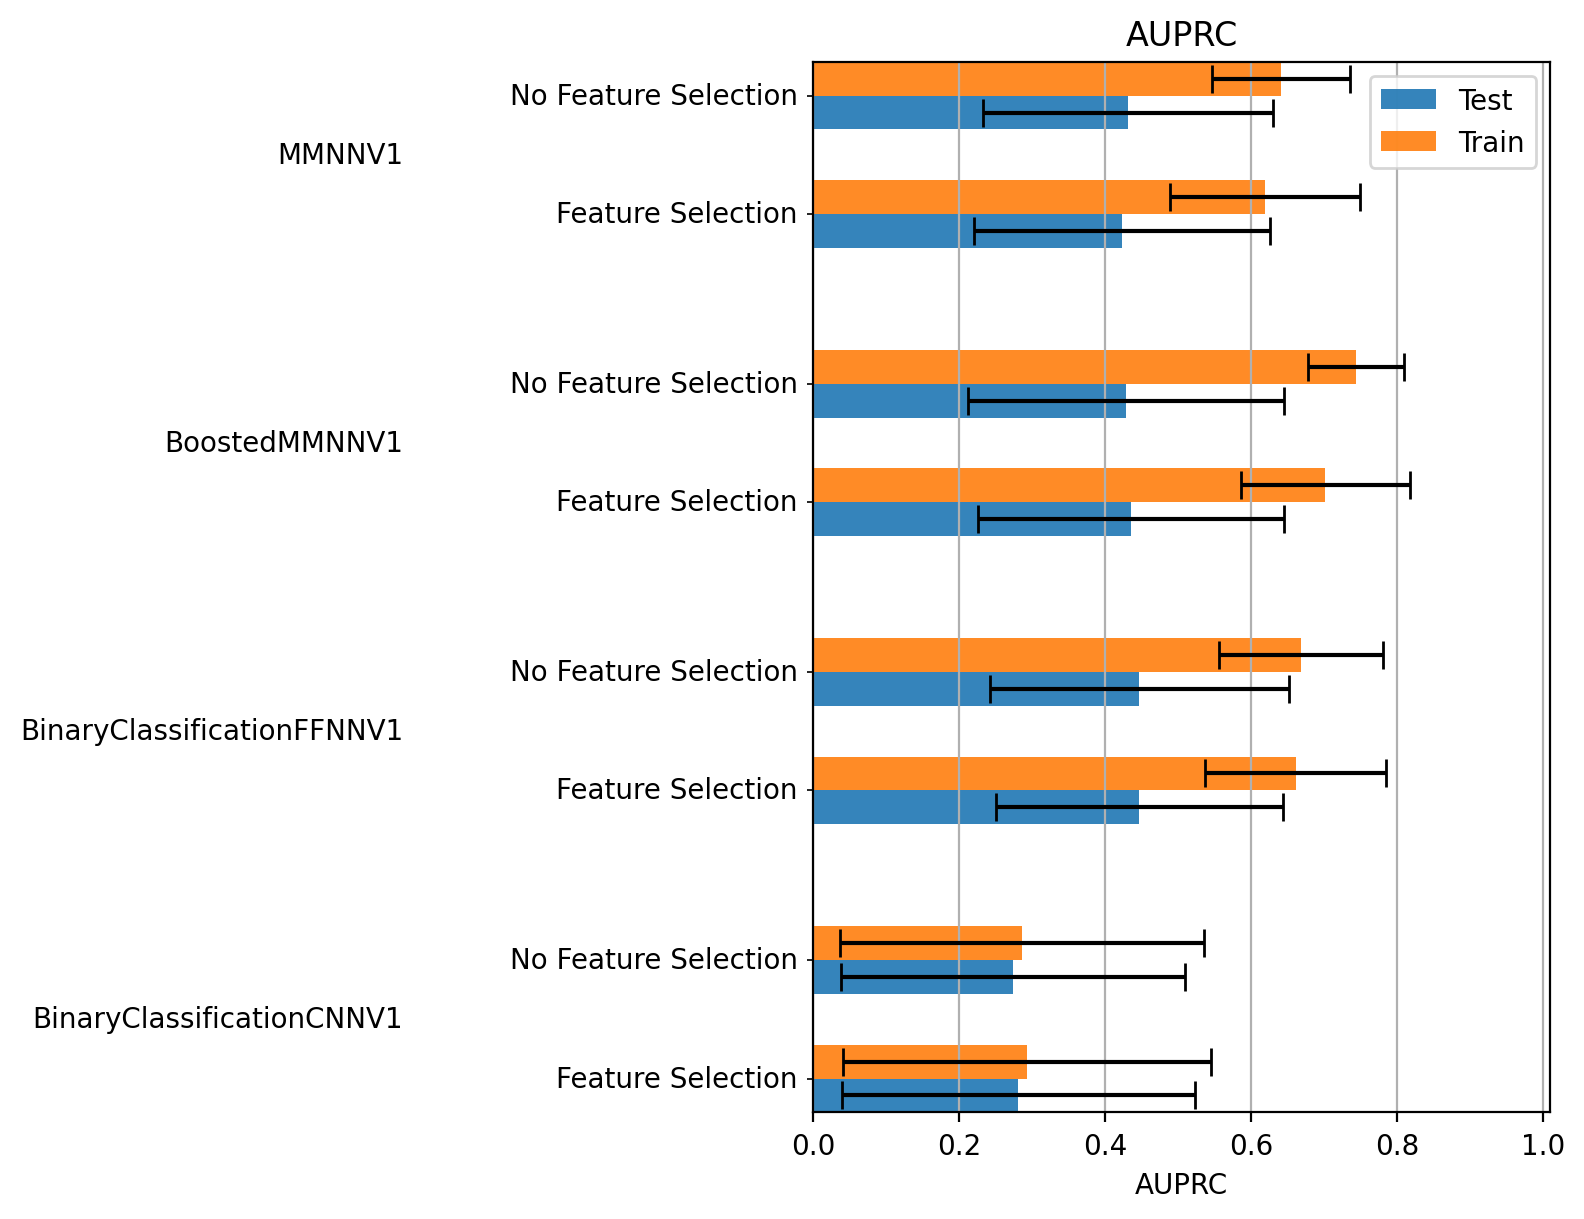
\includegraphics[width=11cm]{image/barplots/enhancers/AUPRC_enhancers.PNG}
        \caption{AUPRC Enhancers}
        \label{fig:AUPRC_enhancers}
    \end{figure}
    \begin{figure}[!ht]
        \centering
        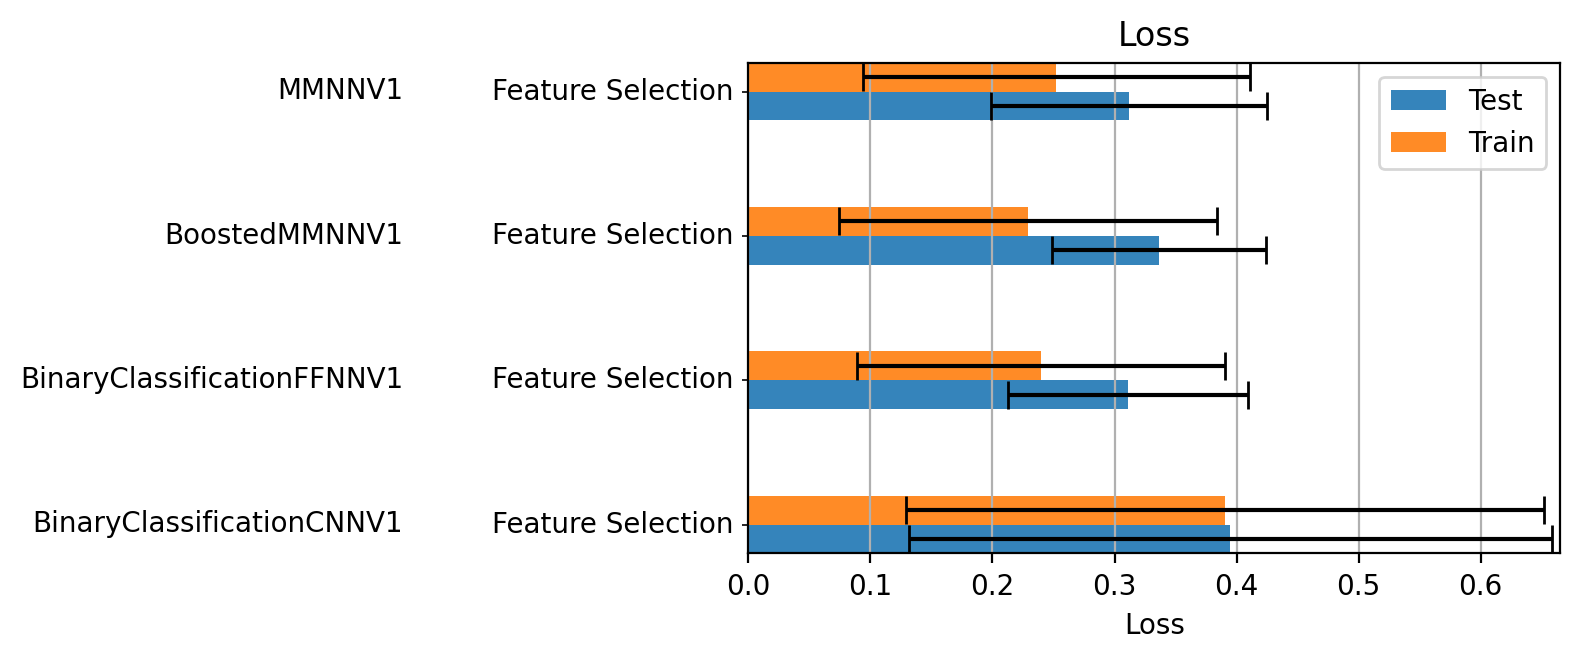
\includegraphics[width=11cm]{image/barplots/promoters/Loss_promoters.PNG}
        \caption{Loss Promoters}
        \label{fig:Loss_promoters}
    \end{figure}
    \begin{figure}[!ht]
        \centering
        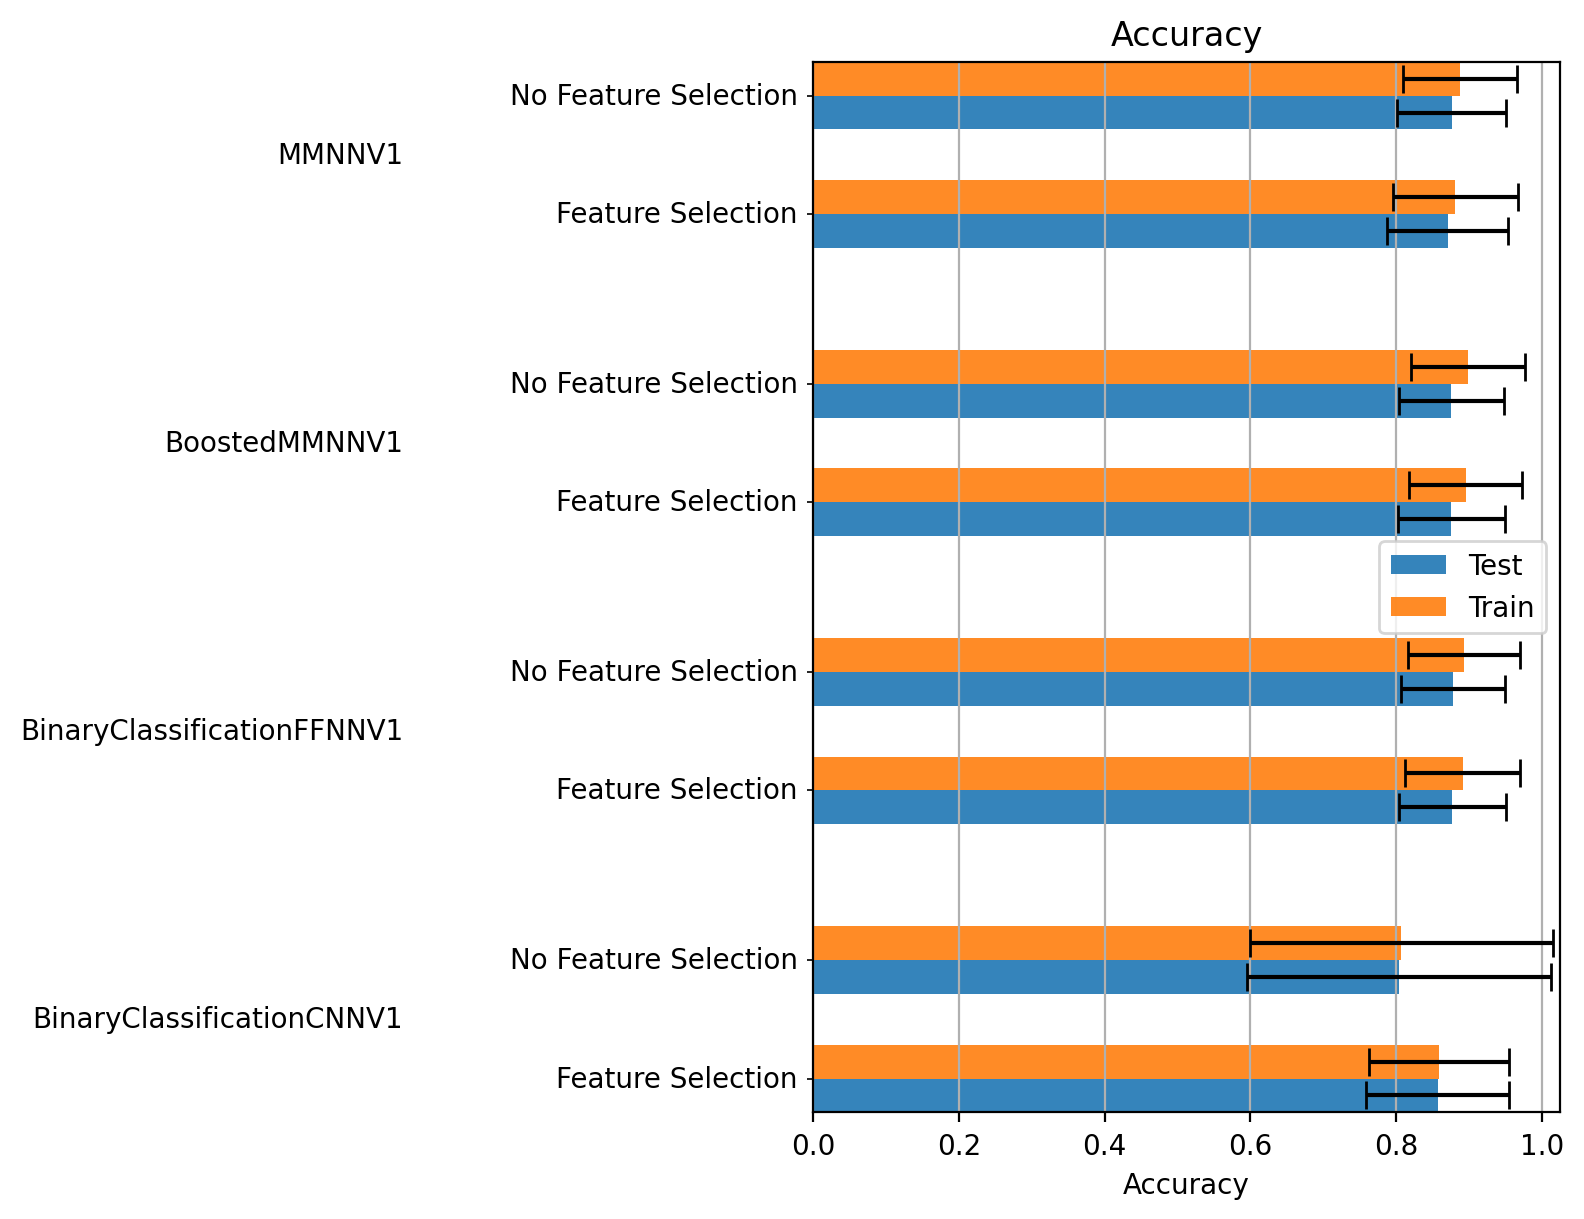
\includegraphics[width=11cm]{image/barplots/promoters/Accuracy_promoters.PNG}
        \caption{Accuracy Promoters}
        \label{fig:Accuracy_promoters}
    \end{figure}
    \begin{figure}[!ht]
        \centering
        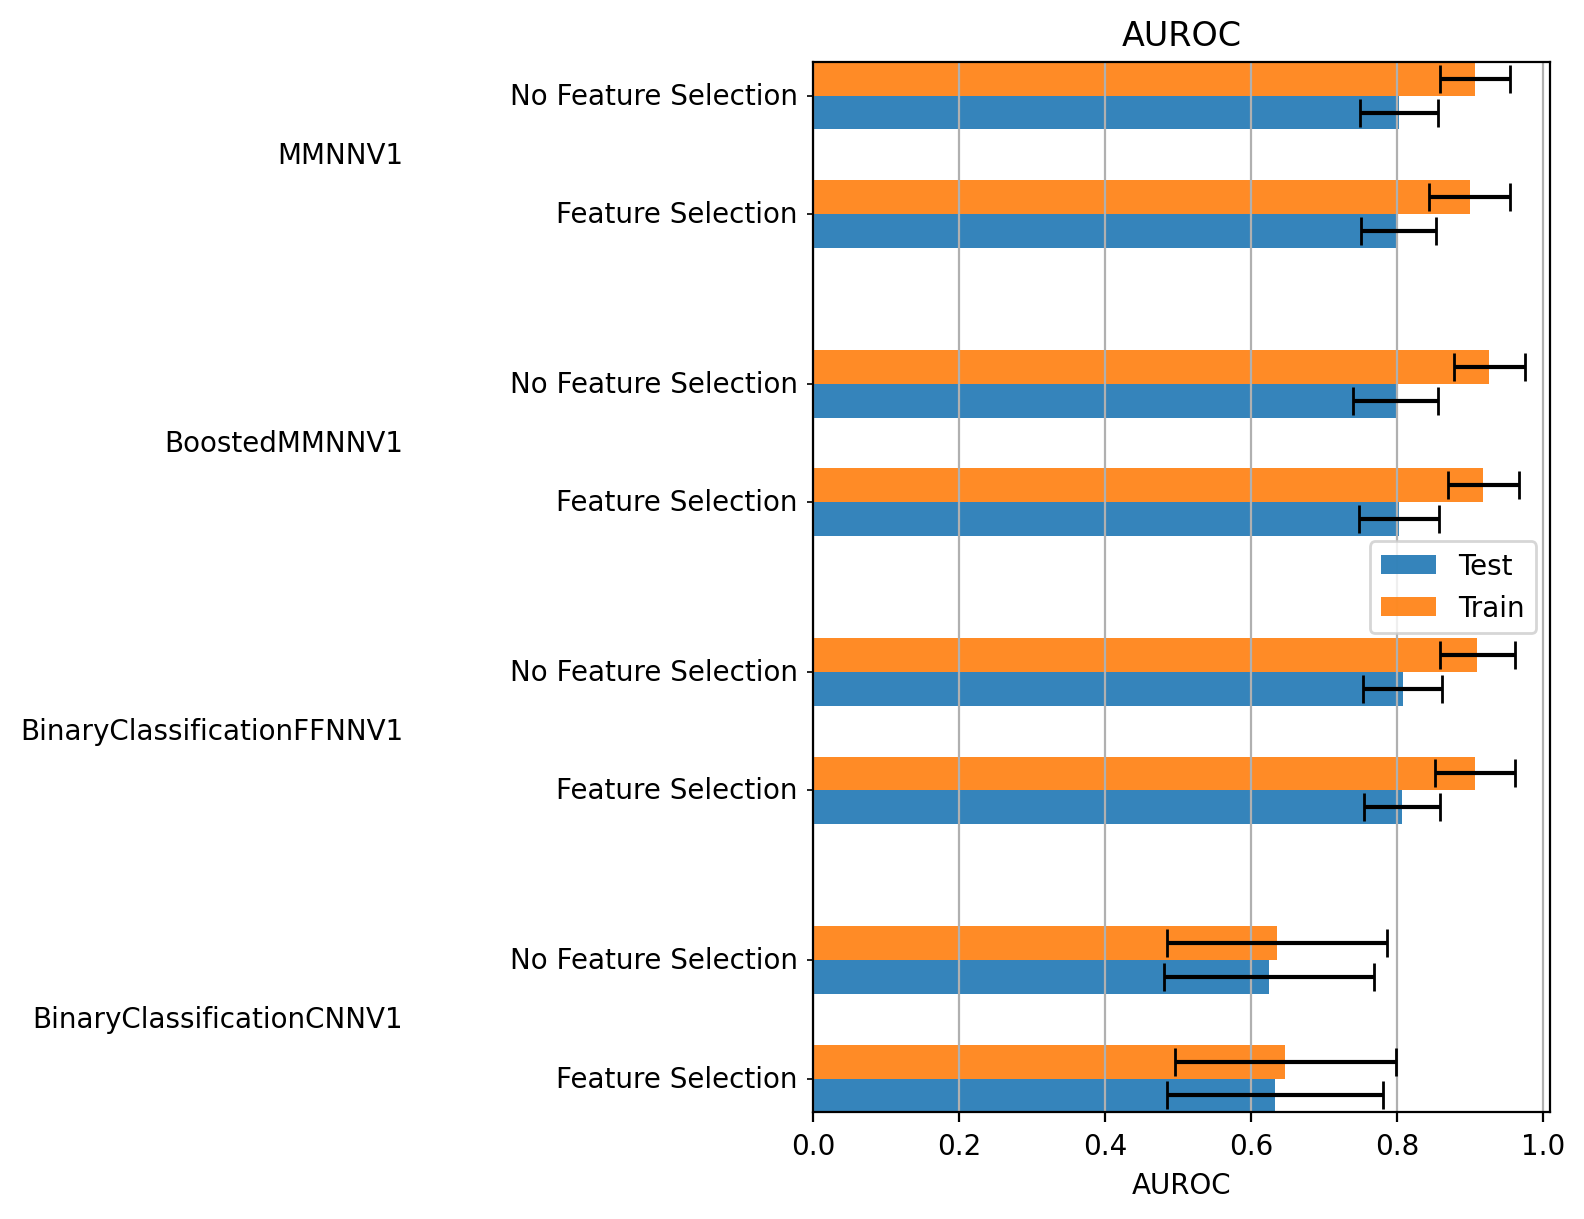
\includegraphics[width=11cm]{image/barplots/promoters/AUROC_promoters.PNG}
        \caption{AUROC Promoters}
        \label{fig:AUROC_promoters}
    \end{figure}
    \begin{figure}[!ht]
        \centering
        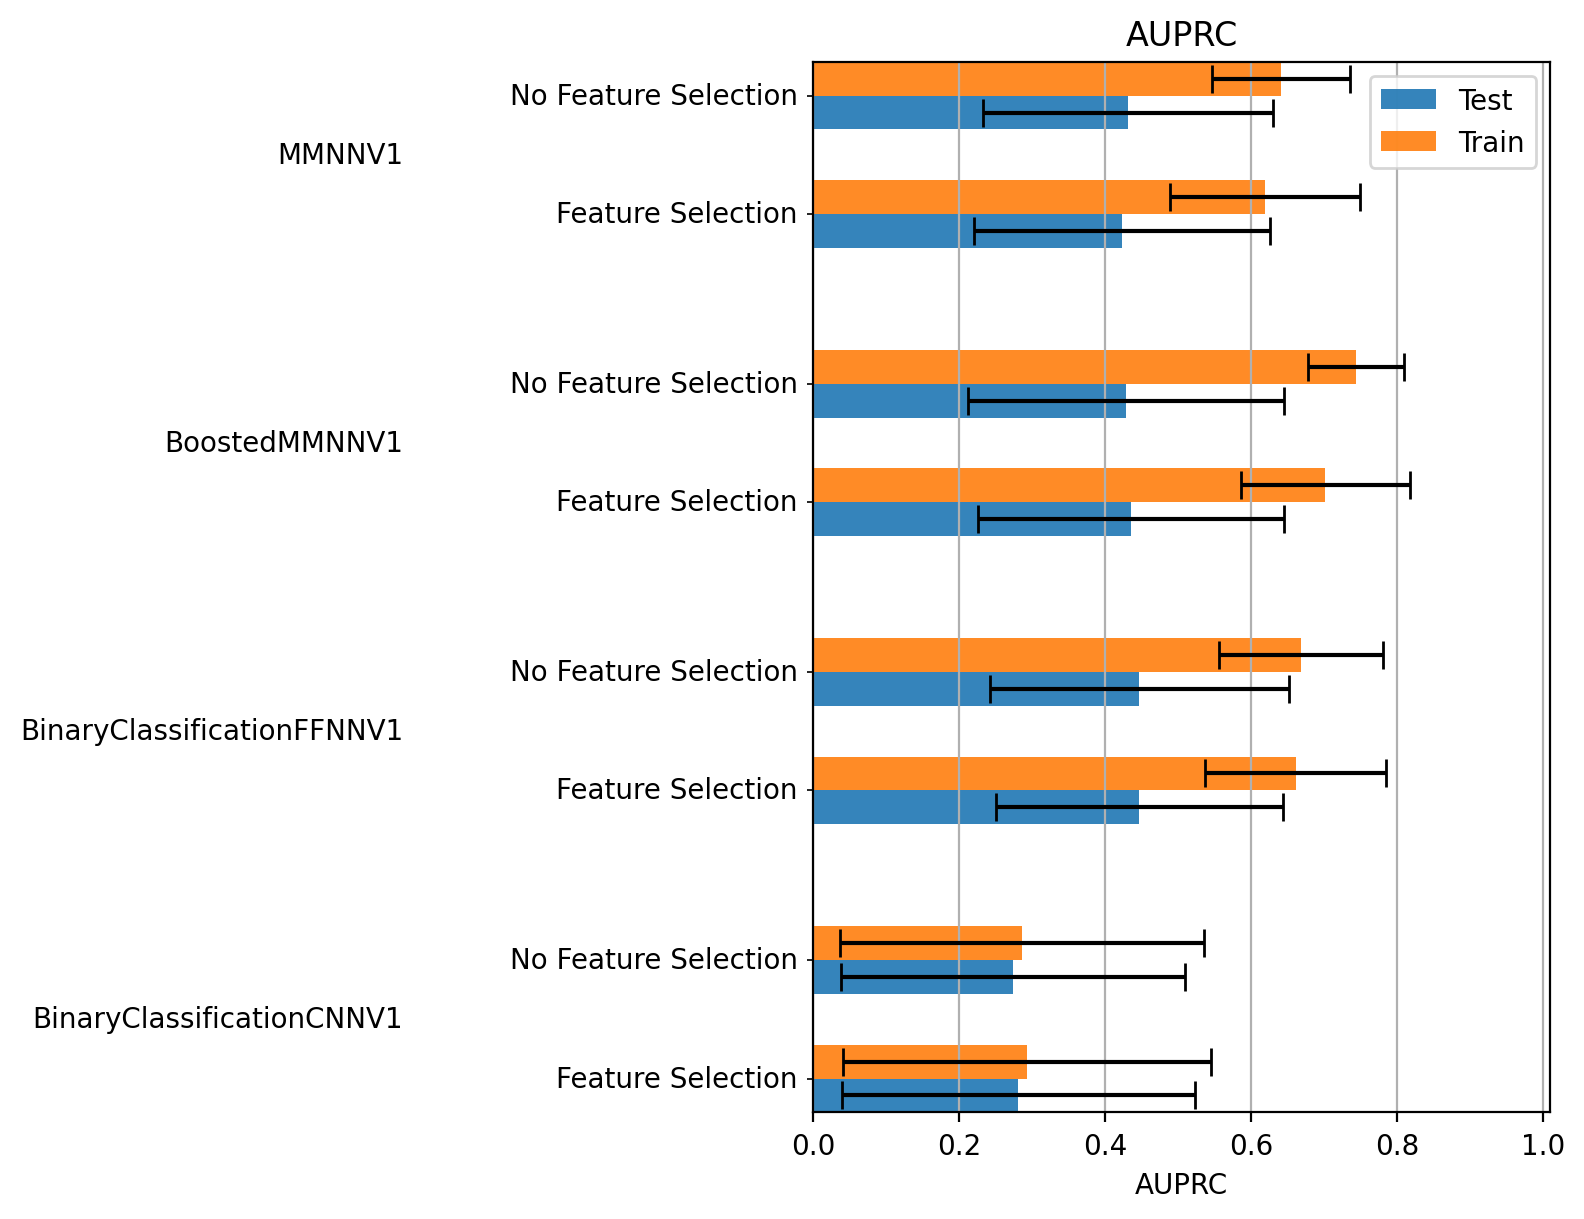
\includegraphics[width=11cm]{image/barplots/promoters/AUPRC_promoters.PNG}
        \caption{AUPRC Promoters}
        \label{fig:AUPRC_promoters}
    \end{figure}
    
    \begin{figure}[!ht]
        \centering
        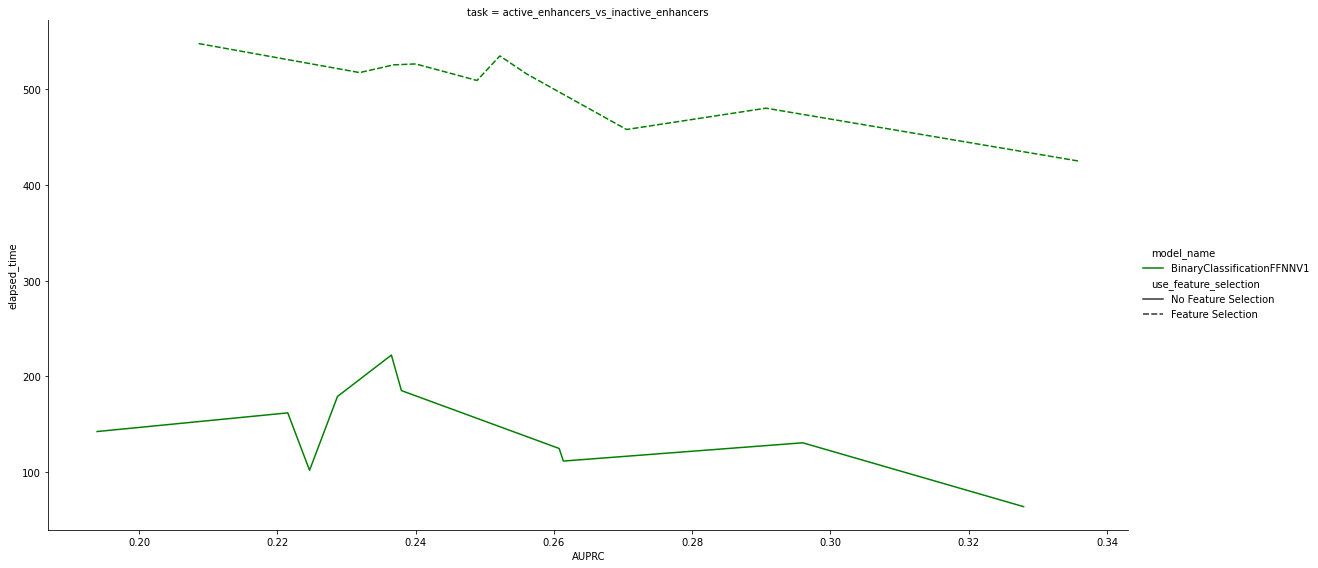
\includegraphics[width=8cm]{image/boruta/enhancers/BinaryClassificationFFNNV1.PNG}
        \caption{Boruta Elapsed Time VS AUPRC On FFNN In Enhancers Task}
        \label{fig:Boruta_enhancers_BinaryClassificationFFNNV1}
    \end{figure}
    \begin{figure}[!ht]
        \centering
        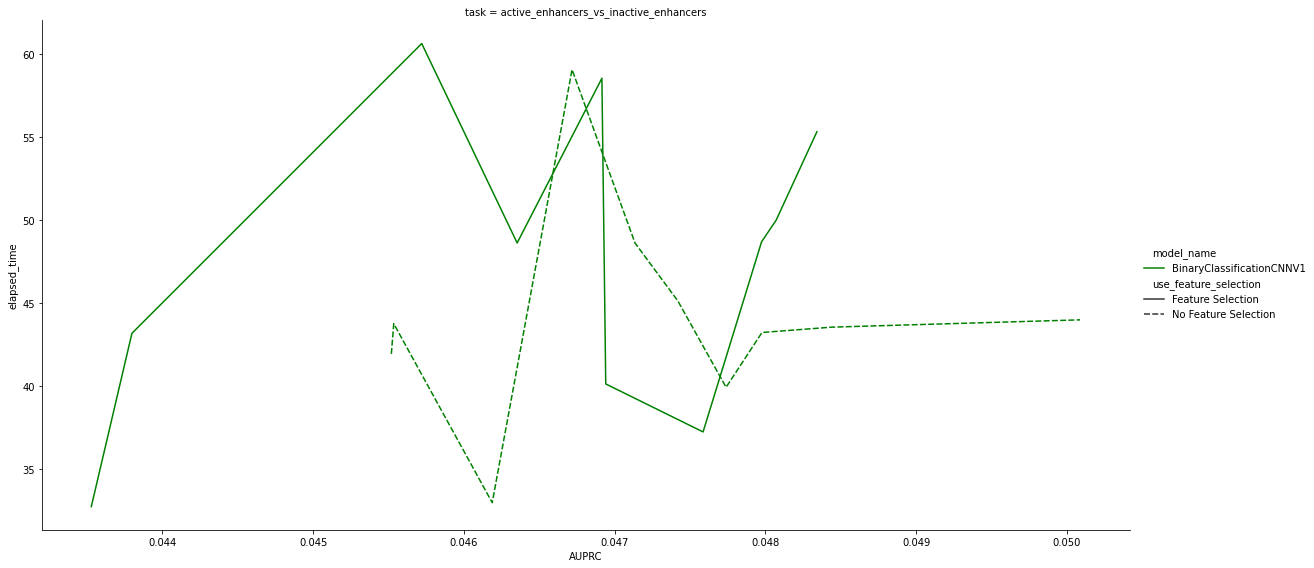
\includegraphics[width=8cm]{image/boruta/enhancers/BinaryClassificationCNNV1.PNG}
        \caption{Boruta Elapsed Time VS AUPRC On CNN In Enhancers Task}
        \label{fig:Boruta_enhancers_BinaryClassificationCNNV1}
    \end{figure}
    \begin{figure}[!ht]
        \centering
        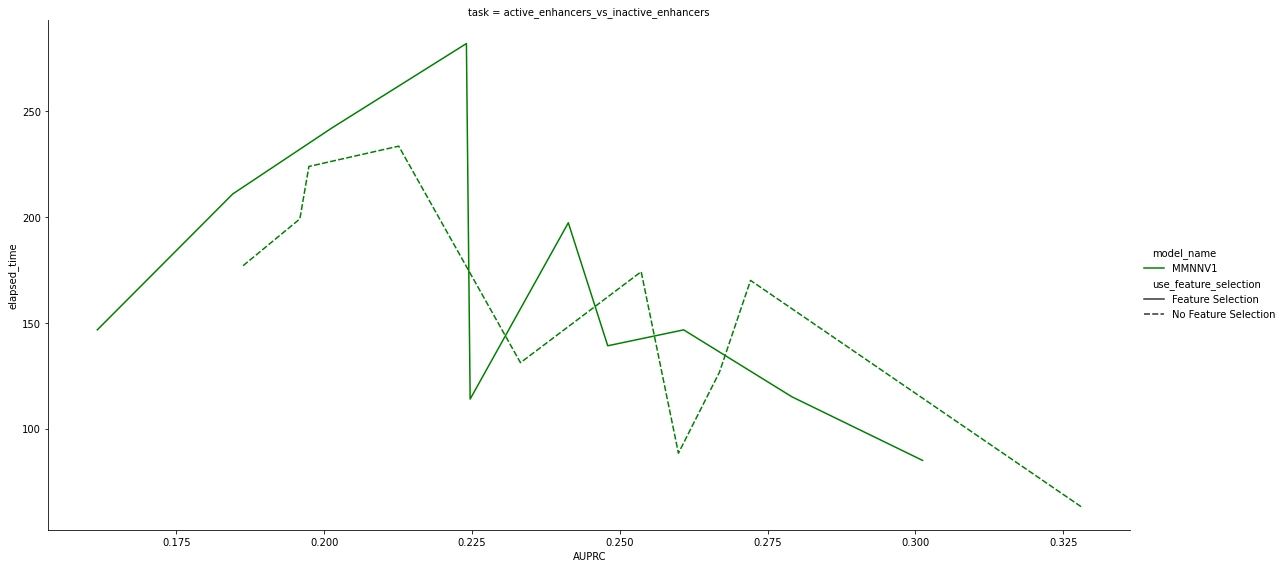
\includegraphics[width=8cm]{image/boruta/enhancers/MMNNV1.PNG}
        \caption{Boruta Elapsed Time VS AUPRC On MMNN In Enhancers Task}
        \label{fig:Boruta_enhancers_MMNNV1}
    \end{figure}
    \begin{figure}[!ht]
        \centering
        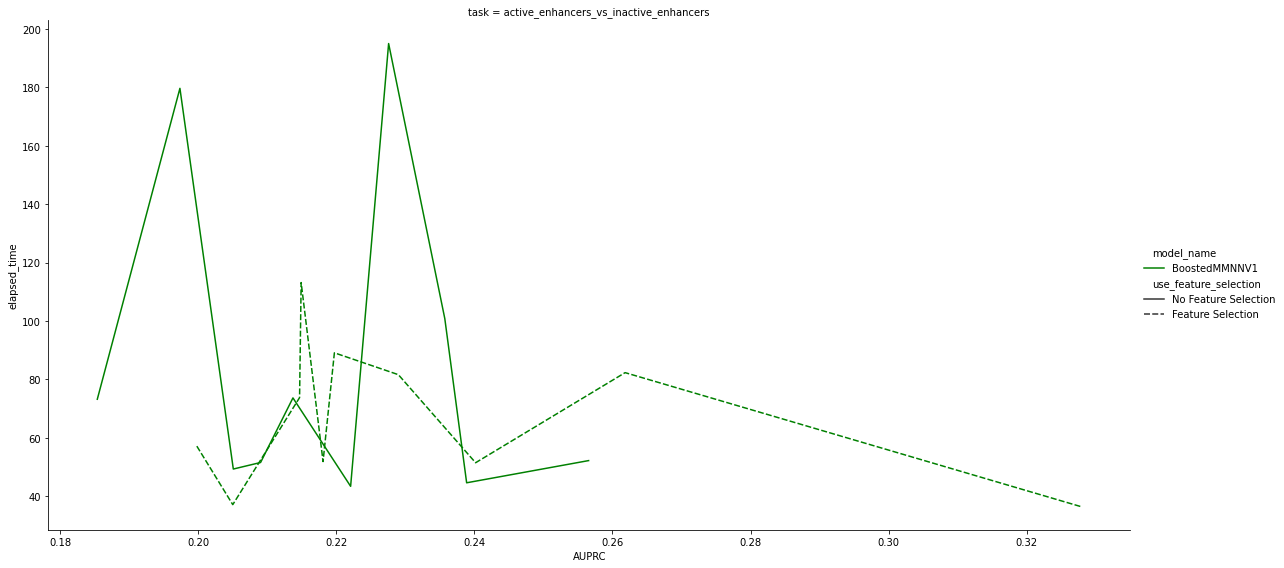
\includegraphics[width=8cm]{image/boruta/enhancers/BoostedMMNNV1.PNG}
        \caption{Boruta Elapsed Time VS AUPRC On Boosted MMNN In Enhancers Task}
        \caption{AUPRC Promoters}
        \label{fig:Boruta_enhancers_BoostedMMNNV1}
    \end{figure}
    
    \begin{figure}[!ht]
        \centering
        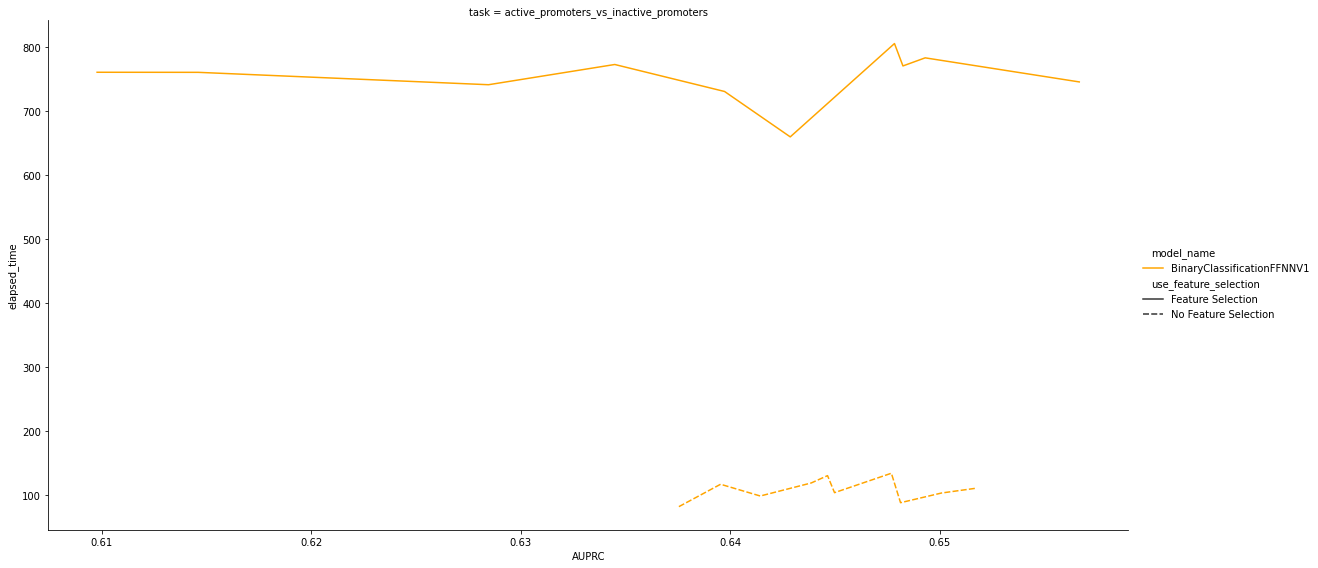
\includegraphics[width=8cm]{image/boruta/promoters/BinaryClassificationFFNNV1.PNG}
        \caption{Boruta Elapsed Time VS AUPRC On FFNN In Promoters Task}
        \label{fig:Boruta_promoters_BinaryClassificationFFNNV1}
    \end{figure}
    \begin{figure}[!ht]
        \centering
        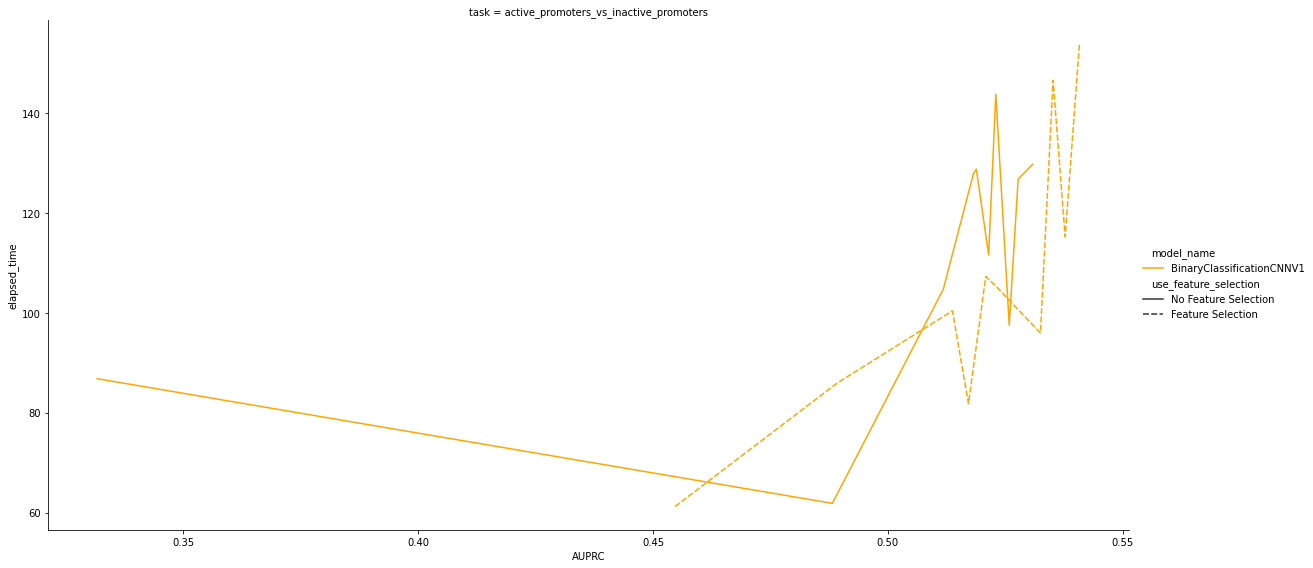
\includegraphics[width=8cm]{image/boruta/promoters/BinaryClassificationCNNV1.PNG}
        \caption{Boruta Elapsed Time VS AUPRC On CNN In Promoters Task}
        \label{fig:Boruta_promoters_BinaryClassificationCNNV1}
    \end{figure}
    \begin{figure}[!ht]
        \centering
        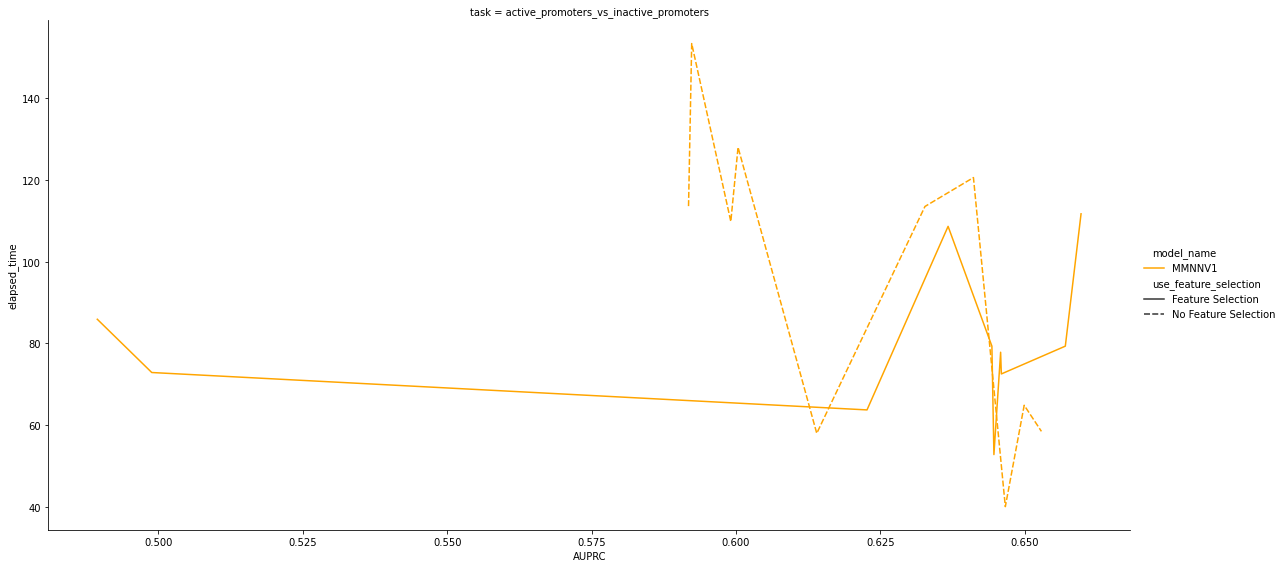
\includegraphics[width=8cm]{image/boruta/promoters/MMNNV1.PNG}
        \caption{Boruta Elapsed Time VS AUPRC On MMNN In Promoters Task}
        \label{fig:Boruta_promoters_MMNNV1}
    \end{figure}
    \begin{figure}[!ht]
        \centering
        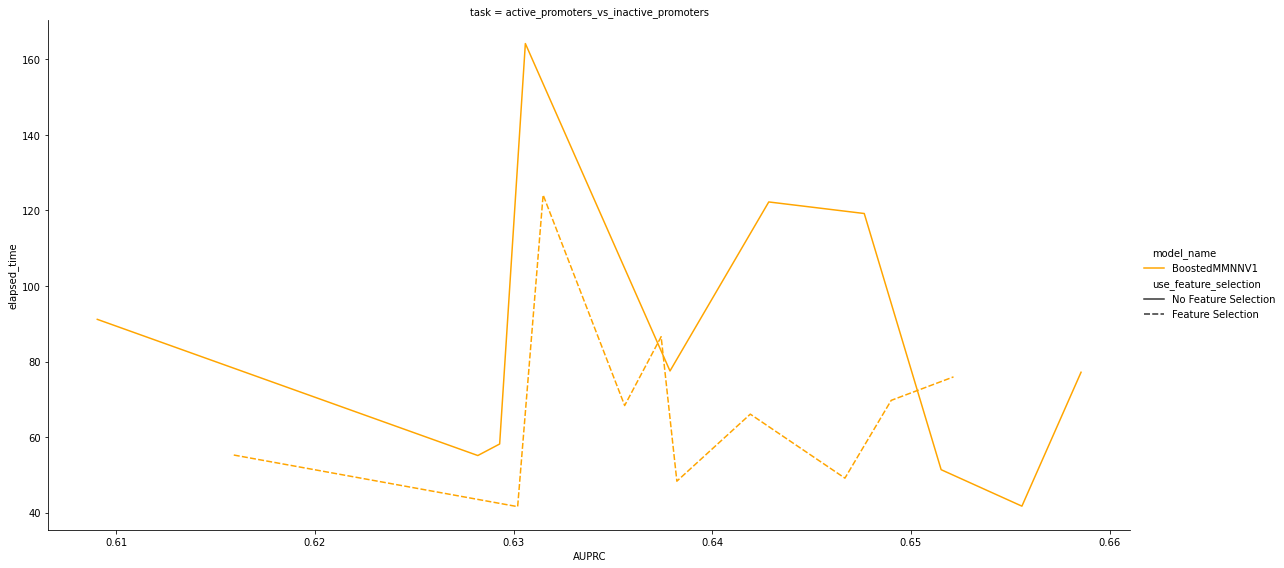
\includegraphics[width=8cm]{image/boruta/promoters/BoostedMMNNV1.PNG}
        \caption{Boruta Elapsed Time VS AUPRC On Boosted MMNN In Promoters Task}
        \label{fig:Boruta_promoters_BoostedMMNNV1}
    \end{figure}
\end{enumerate}

\section{Conclusion}
\label{sec:Conclusion}
A conclusion, by analyzing the plots obtained we can draw conclusions, referring in a precise way to the results shown for the AUPRC metric, which turned out to be the most reliable together with the AUROC, when dealing with problems with unbalanced classes in which you are very interested in finding the positive examples. Surely among all the models, the one that performed best for both tasks was the Multimodal Neural Network, which as described combines the properties of the models making the most of the peculiarities of each of them. It's also visible from these graphs that the help of the feature selection did not affect the performance trend, and it's also necessary to make a note, as regards the CNN model, the differentiation between feature selection and no features selection it's only for the convenience of using the tool for the creation of plotbars, in fact with this model no feature selection has been made, since it uses the sequence data as the first thing, and as a second boruta it has been applied only to epigenomic data, also because applying it to the sequence data is a very complex task that was analyzed in a study \cite{computers9020037} conducted by the research group of Anacleto Lab \footnote{\url{https://anacletolab.di.unimi.it/}}. Probably an easy way to conduct a feature selection on the sequence data and then get different results would have been to vary the windows size, but system limitations and the high amount of task execution time was not explored. It's also possible (as initially expected) to see how the imbalance of the samples related to the enhancers turned out to be crucial for the model training phase, the few samples make learning difficult and tend to overfit the model as can be seen by comparing Figure \ref{fig:AUPRC_enhancers} and Figure \ref{fig:Accuracy_enhancers} where we have a very high accuracy and also a fairly low loss Figure \ref{fig:Loss_enhancers} but a practically almost zero AUPRC. On the other hand, the task relating to promoters is totally different, with a certainly higher number of samples, and a tolerable imbalance between positives and negatives that allows us, with the same metrics \ref{fig:AUPRC_promoters}, \ref{fig:Accuracy_promoters}, \ref{fig:Loss_promoters} viewed, to assert that the models have provided a much better response. Obviously there are some models, such as convolutional neural networks that are very complex to optimize and that in general are used in tasks that generally involve images. For educational and dissemination purposes, we also add to the document two screens relating to the histories of the best AUPRC for the two tasks.

\begin{figure}[!ht]
    \centering
    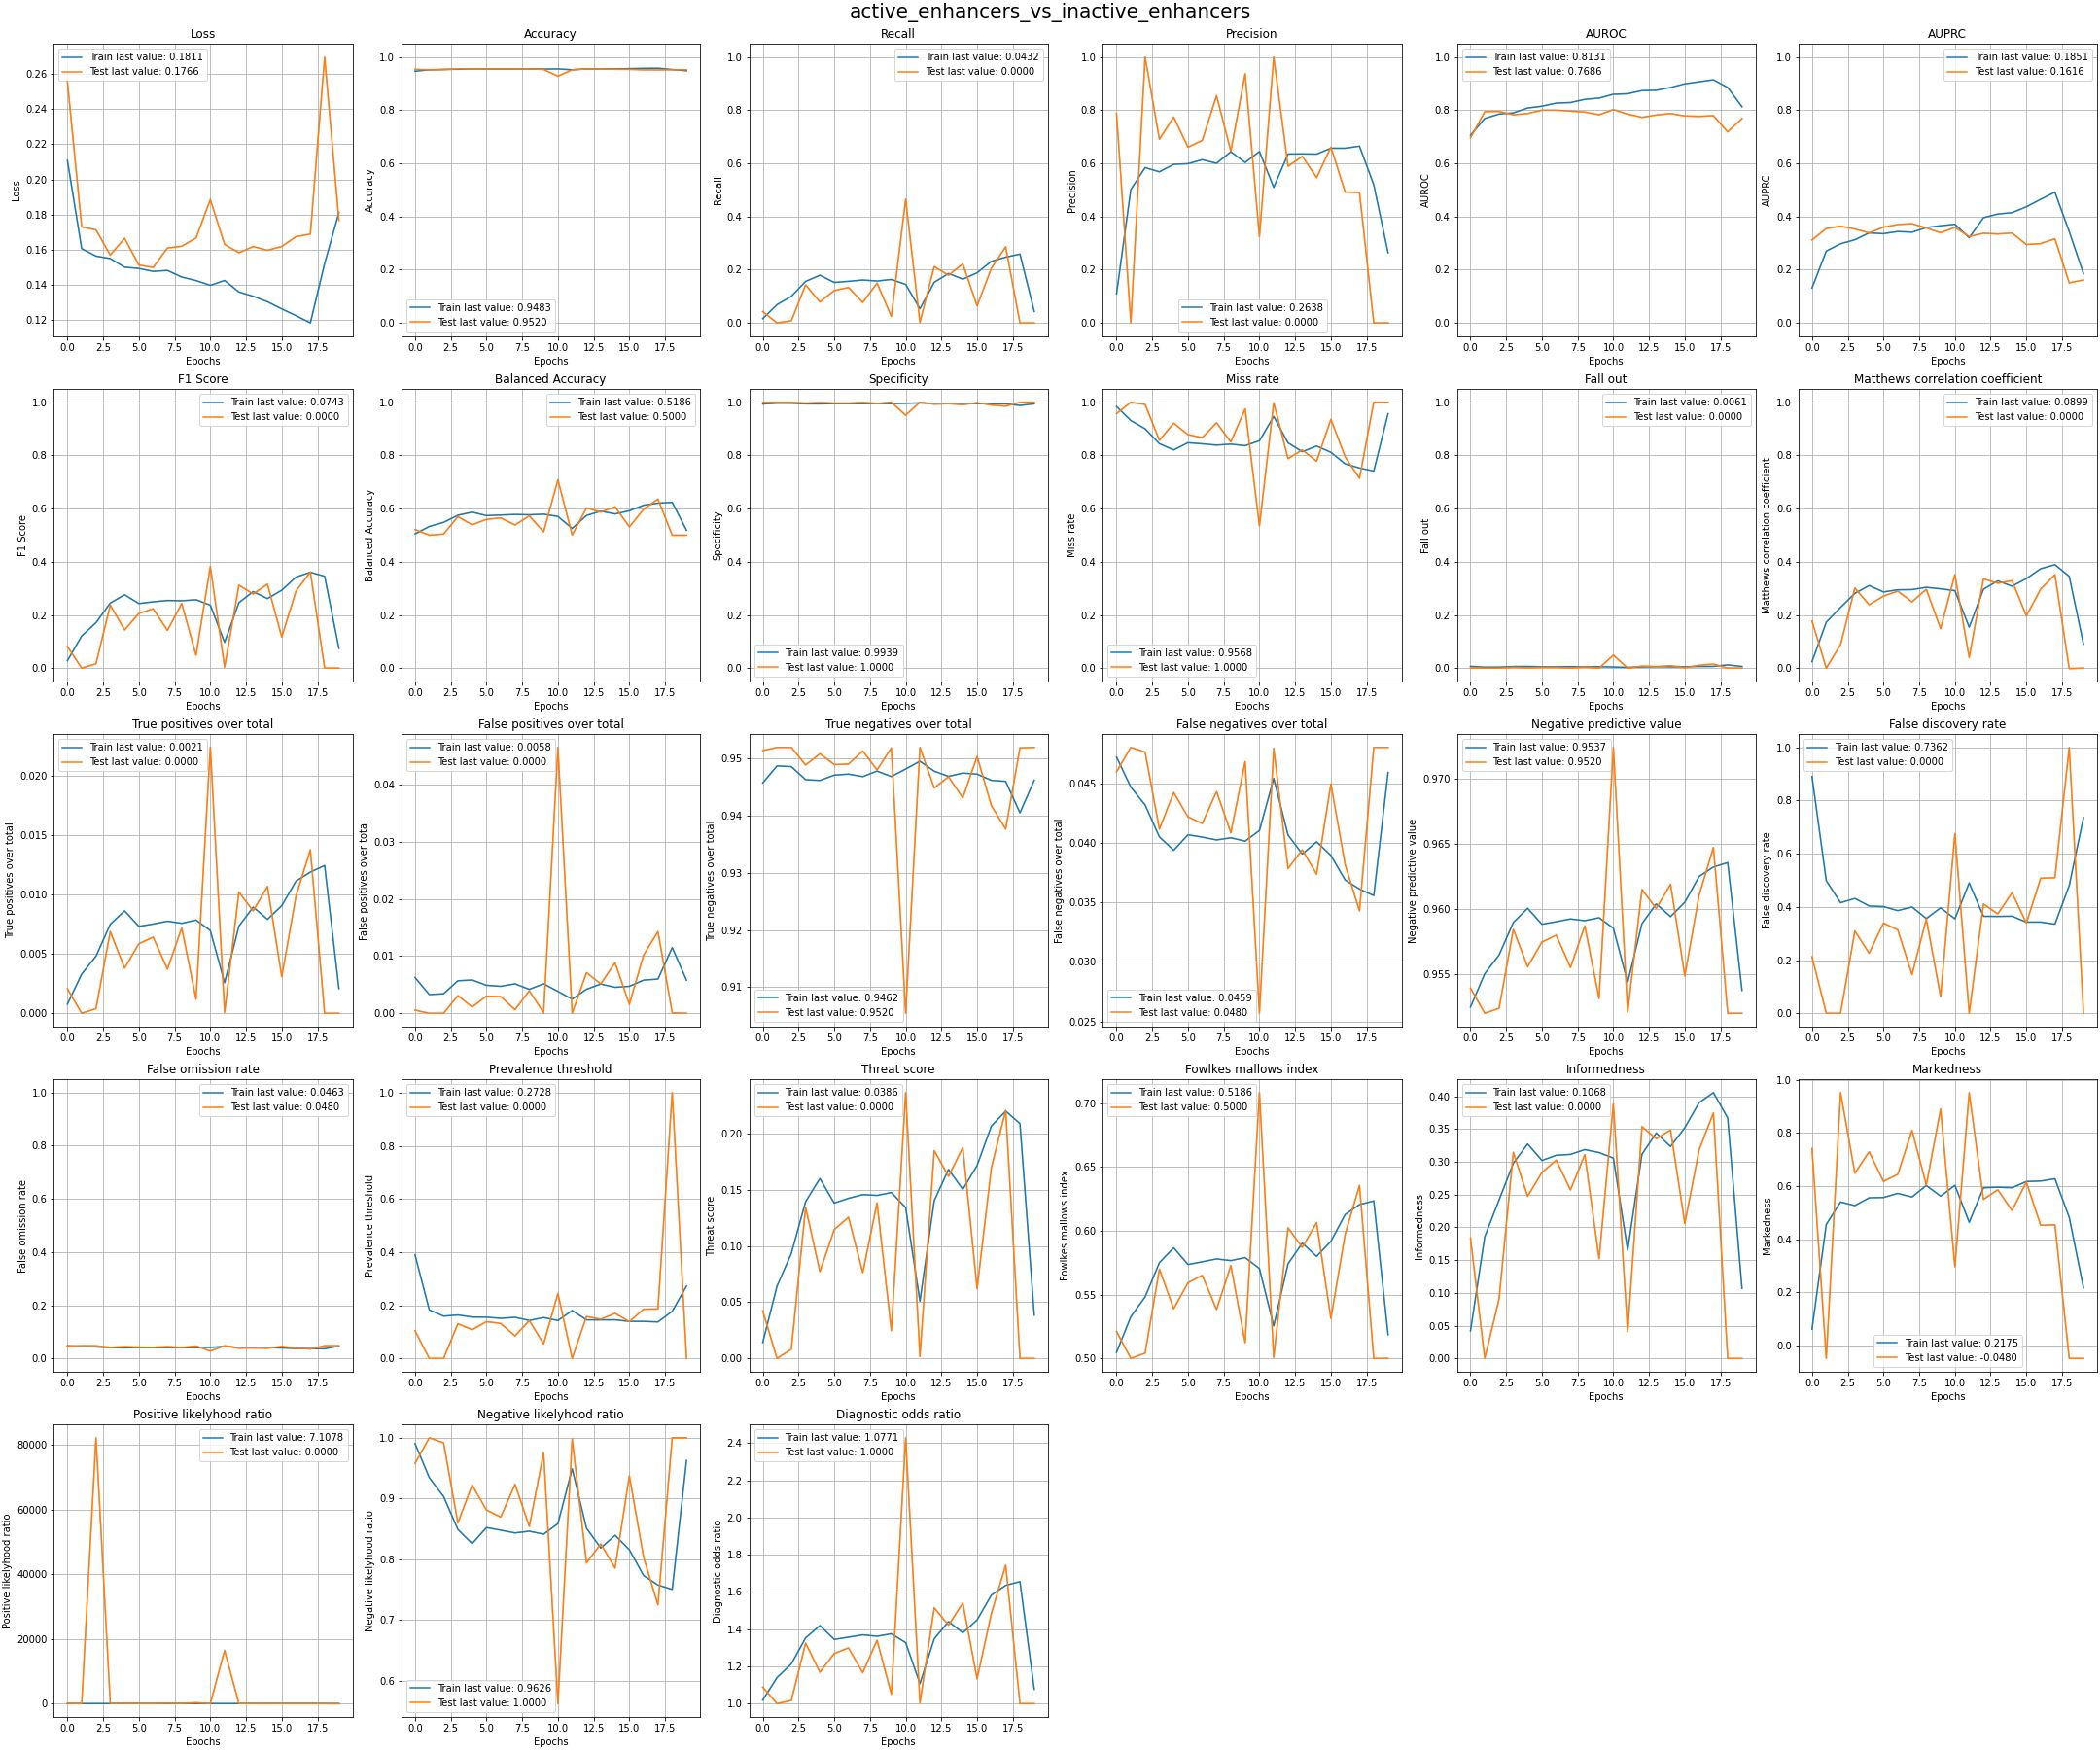
\includegraphics[width=12cm]{image/train_histories/enhancers.PNG}
    \caption{Training Histories Relative At Best AUPRC Value In Enhancers}
    \label{fig:train_histories_enhancers}
\end{figure}
\begin{figure}[!ht]
    \centering
    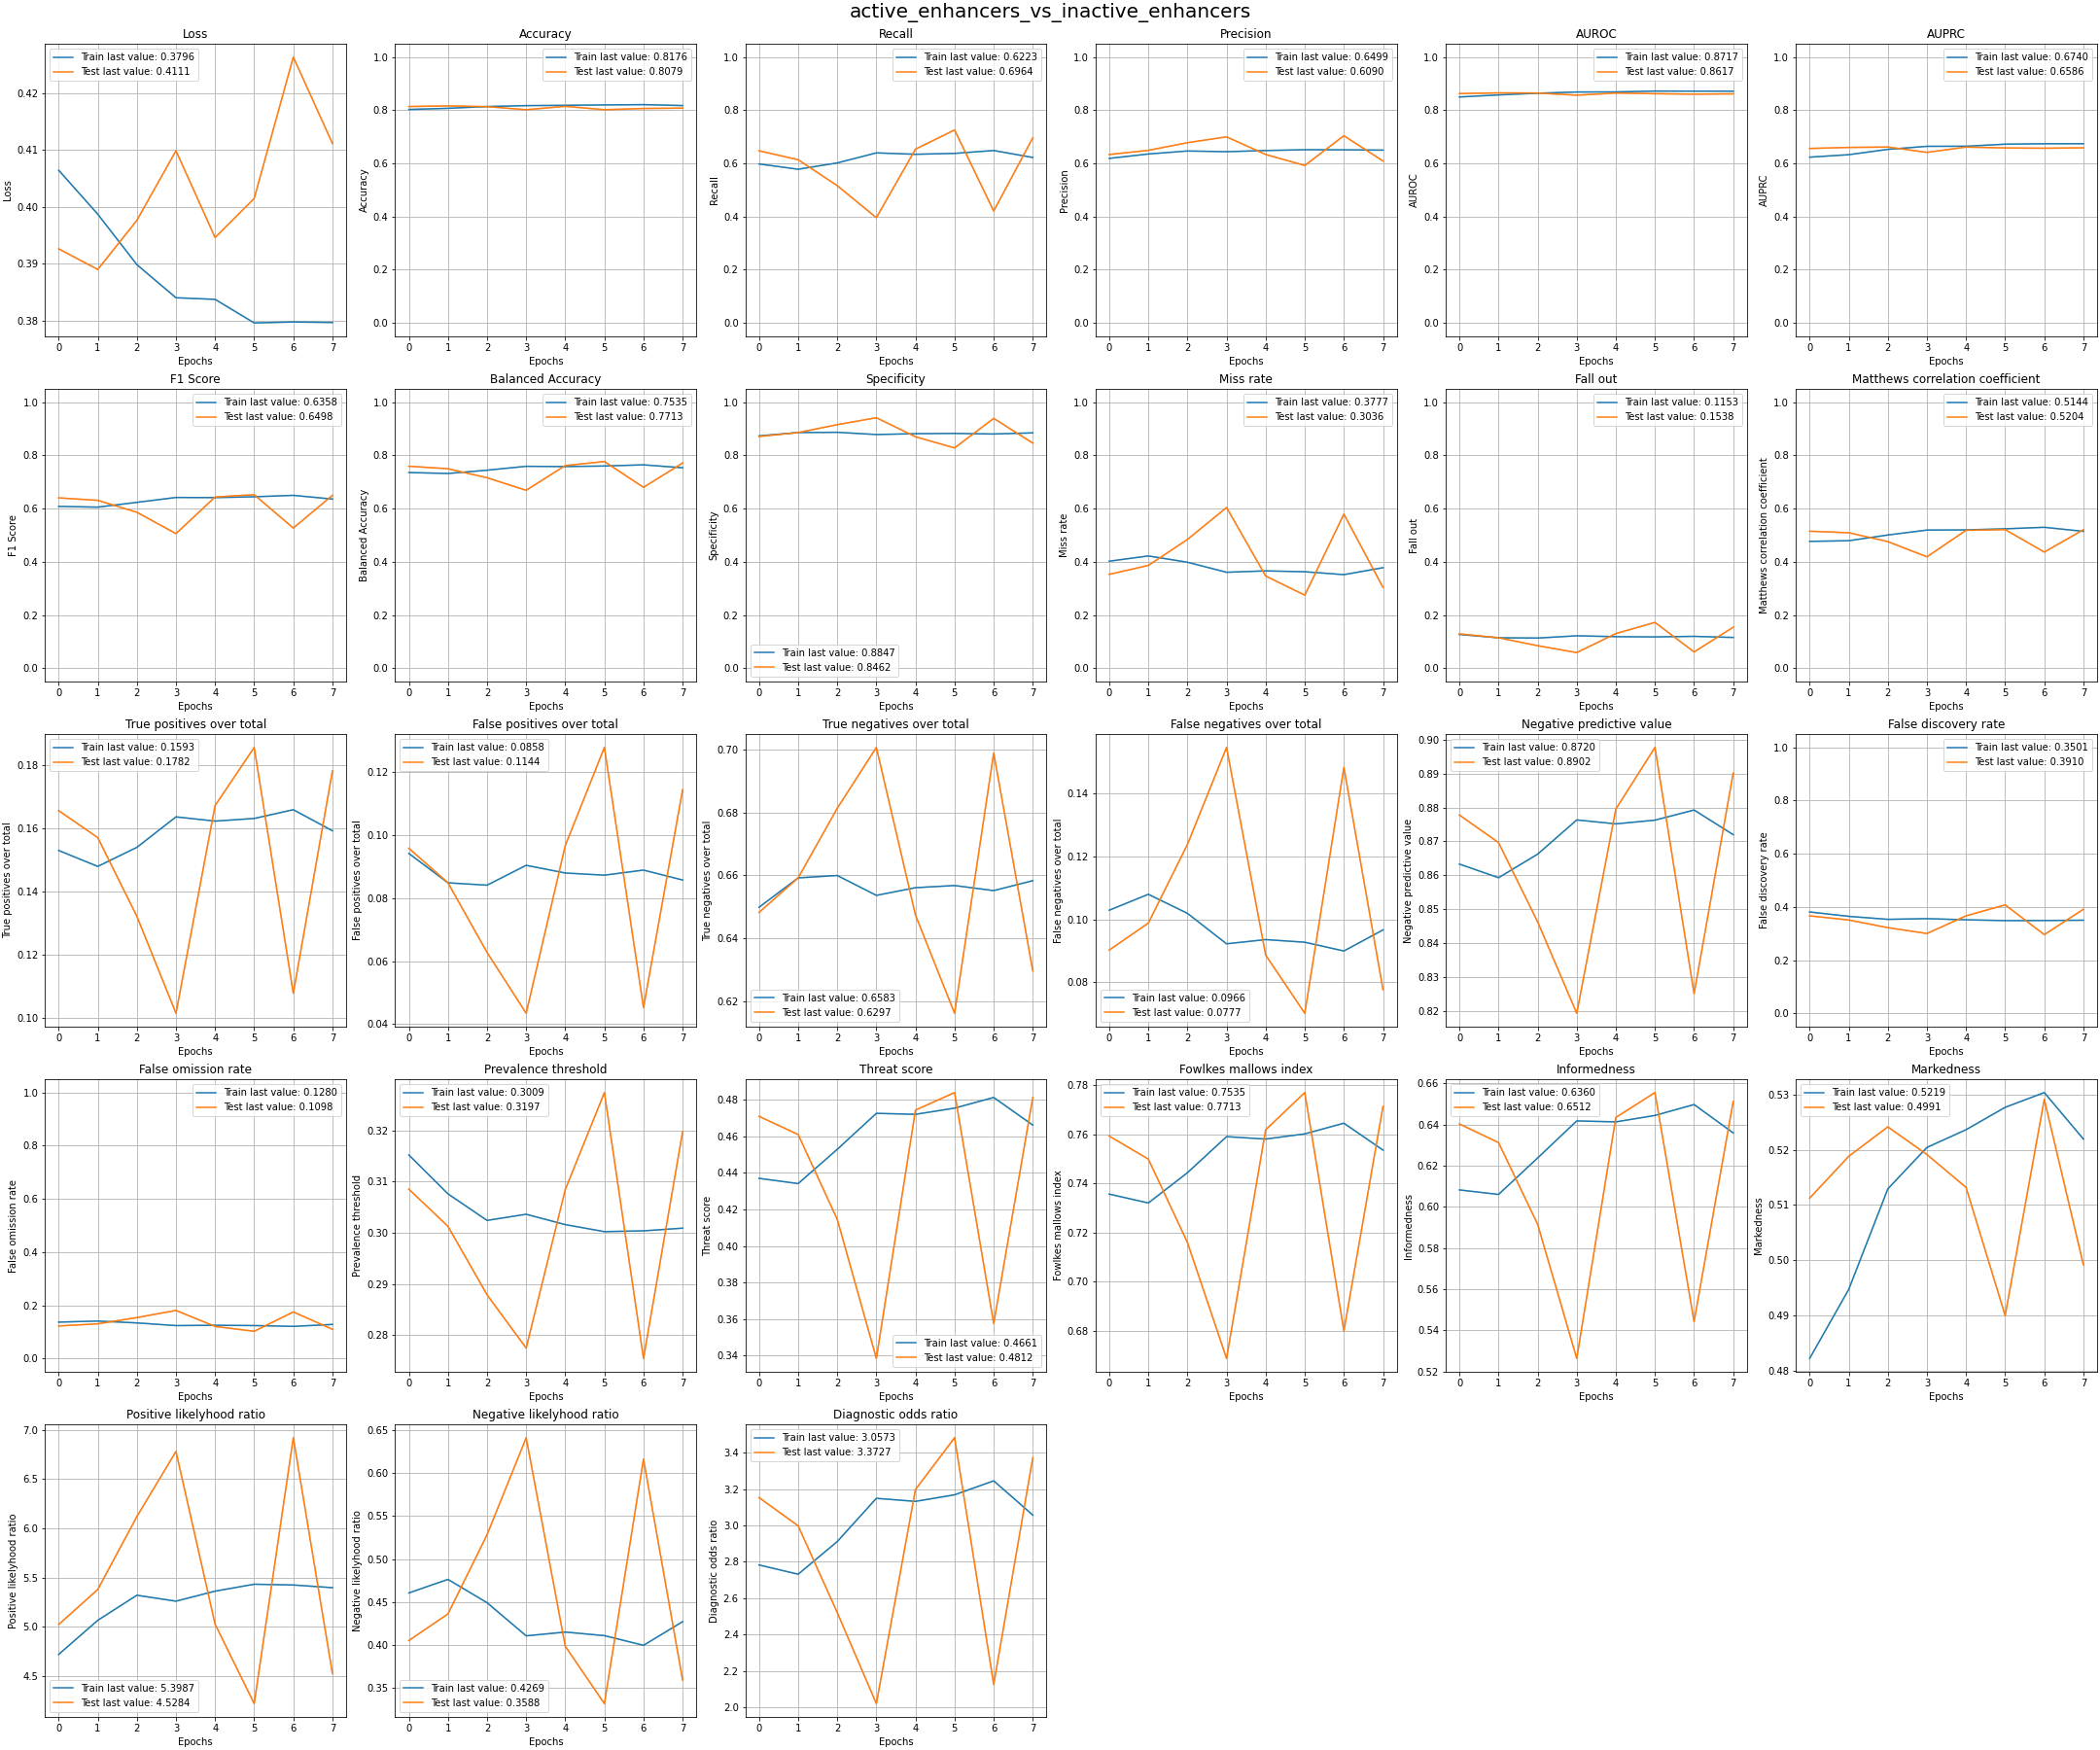
\includegraphics[width=12cm]{image/train_histories/promoters.PNG}
    \caption{Training Histories Relative At Best AUPRC Value In Promoters}
    \label{fig:train_histories_promoters}
\end{figure}

\section{Future Developments}
\label{sec:Future Developments}
We can certainly consider the task analyzed in this problem open and ready to be improved by introducing some corrections and insights. First of all we can try to use meta models based on performing Bayesian algorithms to try to find the best possible model to approach the data in use. Vary the type of models used by, for example, combining in a multimodal network other types of models that are not based on networks but for example on binary trees, such as random forest to see how it behaves with such a complex task. Another thing that we can evaluate while using the convolutional neural network is the combination of the sequence data of the chromosome name with the aid of an embedding layer\footnote{\url{https://www.tensorflow.org/api_docs/python/tf/keras/layers/Embedding}}. It's possible to use techniques such as those introduced by the HyperSMURF\cite{HyperSMURF} algorithm to try to obtain better results in the case of unbalanced classes such as in the enhancers task.

\clearpage
\printglossary[type=\acronymtype]

\bibliographystyle{ieeetr}
\bibliography{references}

\end{document}